
			\level{4}[Model]{Applicazione::Model}
			

		\IfFileExists{DefinizioneDiProdotto/Pics/Classi/Applicazione--Model.pdf}{
			\begin{figure}[H]
				\centering
				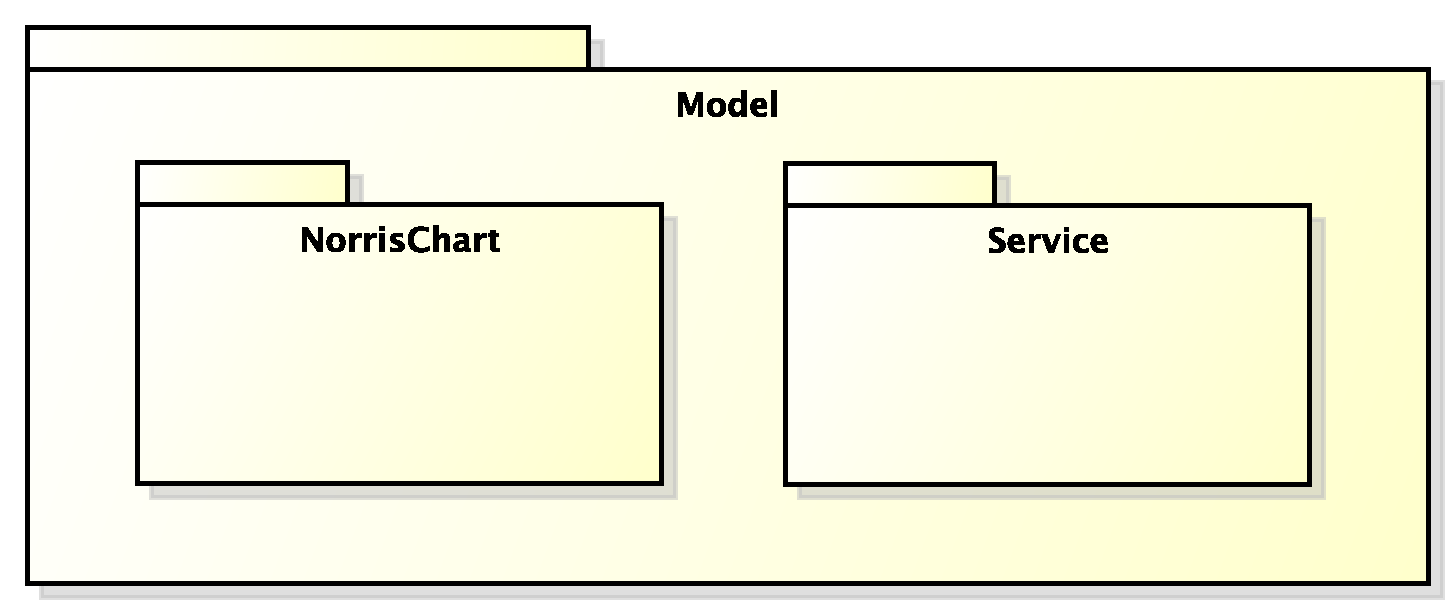
\includegraphics[scale=0.5]{DefinizioneDiProdotto/Pics/Classi/Applicazione--Model}
				\caption{Applicazione::Model}
			\end{figure}
		}
	

			\begin{itemize}
			\item \textbf{Nome:} Model
			\item \textbf{Tipo:} package
			
			\item \textbf{Descrizione:}  Il package Model è un+package%2C+contenente+a+sua+volta%2C+i+package+NorrisChart+e+Service.+Le+classi+del+package+Model+memorizzano+le+informazioni+relative+allo+stato+della+sessione+con+l%27istanza+di+Norris+contenente+i+grafici+che+si+vogliono+visualizzare+con+l%27applicazione.
			\end{itemize}

			
			\level{4}[NorrisChart]{Applicazione::Model::NorrisChart}
			

		\IfFileExists{DefinizioneDiProdotto/Pics/Classi/Applicazione--Model--NorrisChart.pdf}{
			\begin{figure}[H]
				\centering
				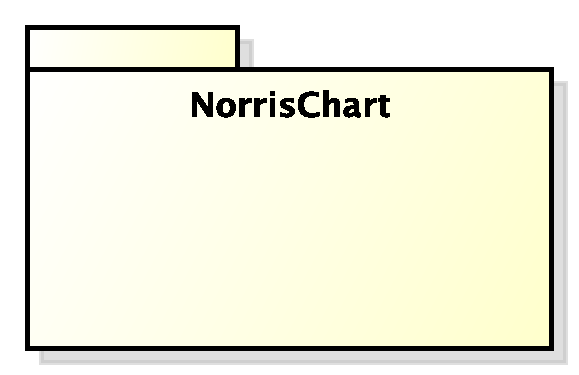
\includegraphics[scale=0.5]{DefinizioneDiProdotto/Pics/Classi/Applicazione--Model--NorrisChart}
				\caption{Applicazione::Model::NorrisChart}
			\end{figure}
		}
	

			\begin{itemize}
			\item \textbf{Nome:} NorrisChart
			\item \textbf{Tipo:} package
			
			\item \textbf{Descrizione:} NorrisChart è il package, le cui classi contengono i dati riguardanti i grafici con le relative impostazioni. Contiene le classi per ogni tipo di grafico, nelle quali sono implementati i metodi, per inserire i dati e configurare le impostazioni, e per ottenere tali valori. Inoltre, le classi di questo package mettono a disposizione le stesse modalità di aggiornamento dei grafici di Norris.
			\end{itemize}

			
			\level{5}[BarChartImpl]{Applicazione::Model::NorrisChart::BarChartImpl}
			

		\IfFileExists{DefinizioneDiProdotto/Pics/Classi/Applicazione--Model--NorrisChart--BarChartImpl.pdf}{
			\begin{figure}[H]
				\centering
				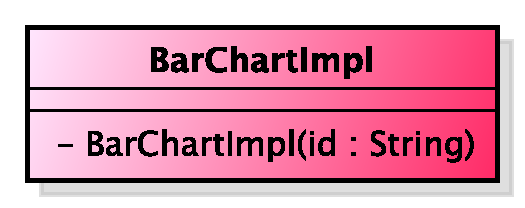
\includegraphics[scale=0.5]{DefinizioneDiProdotto/Pics/Classi/Applicazione--Model--NorrisChart--BarChartImpl}
				\caption{Applicazione::Model::NorrisChart::BarChartImpl}
			\end{figure}
		}
	
			
			\begin{itemize}
			\item \textbf{Nome:} BarChartImpl
			\item \textbf{Tipo:} classe
			
		\item \textbf{Estende:}
		ChartImpl
		\item \textbf{Astratta:}
		no
			\item \textbf{Visibilità:} package
			\item \textbf{Descrizione:} Questa classe rappresenta un grafico di tipo bar chart. Essa contiene al suo interno i dati (BarChartDataObject) e le impostazioni (BarChartSettingsObject) relativi al grafico. Inoltre contiene la classe BarChartInPlaceUpdater, la quale implementa l'aggiornamento di tipo in place per il grafico in questione. Un'istanza della classe BarChartImpl viene creata dalla classe factory BarChartFactory.
			\item \textbf{Metodi:}
				\begin{itemize}
				\setlength{\itemsep}{5pt}
				
					\item[\ding{111}] {{--BarChartImpl(chartId : String)}} \\ [1mm] Tale metodo è il costruttore. Esso è privato perchè non può esser creata una istanza se non dalla sua classe interna factory.
				\end{itemize}
		
			\end{itemize}

			
			\level{5}[BarChartFactory]{Applicazione::Model::NorrisChart::BarChartImpl::BarChartFactory}
			

		\IfFileExists{DefinizioneDiProdotto/Pics/Classi/Applicazione--Model--NorrisChart--BarChartImpl--BarChartFactory.pdf}{
			\begin{figure}[H]
				\centering
				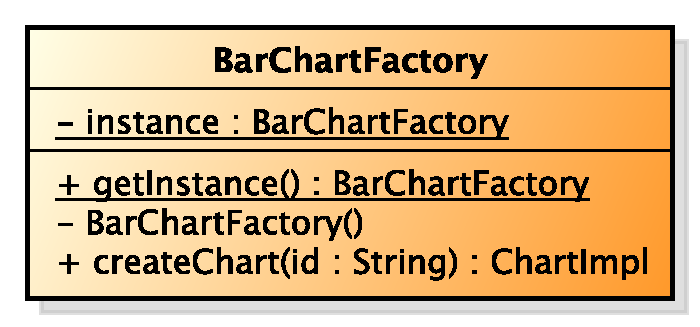
\includegraphics[scale=0.5]{DefinizioneDiProdotto/Pics/Classi/Applicazione--Model--NorrisChart--BarChartImpl--BarChartFactory}
				\caption{Applicazione::Model::NorrisChart::BarChartImpl::BarChartFactory}
			\end{figure}
		}
	
			
			\begin{itemize}
			\item \textbf{Nome:} BarChartFactory
			\item \textbf{Tipo:} classe
			
		\item \textbf{Implementa:}
		ChartFactory
		\item \textbf{Astratta:}
		no
			\item \textbf{Visibilità:} private
			\item \textbf{Descrizione:} Questa classe si occupa della creazione di un grafico di tipo BarChartImpl. In particolare si occupa di configurare i dati e le impostazioni del grafico. Tale classe dispone di un blocco di inizializzazione statica che registra la sua istanza nel HashMap factories della classe ChartImpl non appena tale classe viene caricata.
			\item \textbf{Attributi:}
				\begin{itemize}
				\setlength{\itemsep}{5pt}
				
					\item[\ding{111}] \underline{--instance : BarChartFactory} \\ [1mm] Tale attributo statico rappresenta l'istanza univoca di tale classe.
				\end{itemize}
		
			\item \textbf{Metodi:}
				\begin{itemize}
				\setlength{\itemsep}{5pt}
				
					\item[\ding{111}] {\underline{+getInstance() : ChartFactory}} \\ [1mm] Tale metodo ha il compito di ritornare l'istanza unica di tale classe e se non esiste la crea.
					\item[\ding{111}] {{--BarChartFactory()}} \\ [1mm] Tale metodo è il costruttore della classe. Esso è privato perchè non si vuole permettere a nessuno di poter creare un'istanza se non utilizzando il metodo getInstance().
					\item[\ding{111}] {{+createChart(chartId : String) : ChartImpl}} \\ [1mm] Tale metodo ha il compito di creare la relativa specializzazione di ChartImpl. Esso può accedere al suo costruttore perchè questa classe factory è interna alla relativa classe BarChartImpl.
				\end{itemize}
		
			\end{itemize}

			
			\level{5}[BarChartInPlaceUpdater]{Applicazione::Model::NorrisChart::BarChartInPlaceUpdater}
			

		\IfFileExists{DefinizioneDiProdotto/Pics/Classi/Applicazione--Model--NorrisChart--BarChartInPlaceUpdater.pdf}{
			\begin{figure}[H]
				\centering
				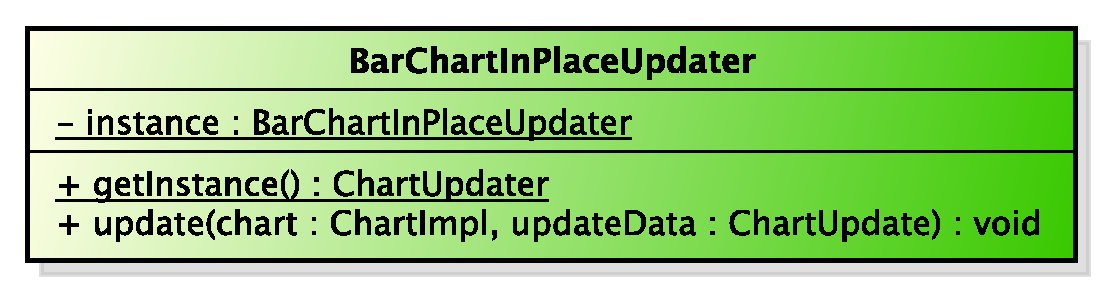
\includegraphics[scale=0.5]{DefinizioneDiProdotto/Pics/Classi/Applicazione--Model--NorrisChart--BarChartInPlaceUpdater}
				\caption{Applicazione::Model::NorrisChart::BarChartInPlaceUpdater}
			\end{figure}
		}
	
			
			\begin{itemize}
			\item \textbf{Nome:} BarChartInPlaceUpdater
			\item \textbf{Tipo:} classe
			
		\item \textbf{Implementa:}
		ChartUpdater
		\item \textbf{Astratta:}
		no
			\item \textbf{Visibilità:} package
			\item \textbf{Descrizione:} Questa classe si occupa di definire il metodo di aggiornamento in place per un grafico di tipo bar chart. Essendo una classe interna di BarChartImpl, ha acceso ai campi dati privati di questa classe. In particolare può accedere al DataObject contenuto in BarChartImpl e modificarne i valori.
			\item \textbf{Attributi:}
				\begin{itemize}
				\setlength{\itemsep}{5pt}
				
					\item[\ding{111}] \underline{--instance : BarChartInPlaceUpdater} \\ [1mm] Tale attributo statico rappresenta l'istanza univoca di tale classe.
				\end{itemize}
		
			\item \textbf{Metodi:}
				\begin{itemize}
				\setlength{\itemsep}{5pt}
				
					\item[\ding{111}] {\underline{+getInstance() : ChartUpdater}} \\ [1mm] Tale metodo ha il compito di ritornare l'istanza unica di tale classe e se non esiste la crea.
					\item[\ding{111}] {{+update(chart : ChartImpl, updateData : ChartUpdate) : void}} \\ [1mm] Tale metodo ha il compito di aggiornare il chart passato come parametro (chart) utilizzando il pacchetto di aggiornamento (updatedata).
				\end{itemize}
		
			\end{itemize}

			
			\level{5}[ChartData]{Applicazione::Model::NorrisChart::ChartData}
			

		\IfFileExists{DefinizioneDiProdotto/Pics/Classi/Applicazione--Model--NorrisChart--ChartData.pdf}{
			\begin{figure}[H]
				\centering
				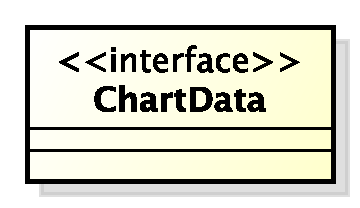
\includegraphics[scale=0.5]{DefinizioneDiProdotto/Pics/Classi/Applicazione--Model--NorrisChart--ChartData}
				\caption{Applicazione::Model::NorrisChart::ChartData}
			\end{figure}
		}
	
			
			\begin{itemize}
			\item \textbf{Nome:} ChartData
			\item \textbf{Tipo:} interfaccia
			
			\item \textbf{Visibilità:} public
			\item \textbf{Descrizione:} ChartData è l'interfaccia delle classi che rappresentano i dati di un grafico.
			\end{itemize}

			
			\level{5}[ChartImpl]{Applicazione::Model::NorrisChart::ChartImpl}
			

		\IfFileExists{DefinizioneDiProdotto/Pics/Classi/Applicazione--Model--NorrisChart--ChartImpl.pdf}{
			\begin{figure}[H]
				\centering
				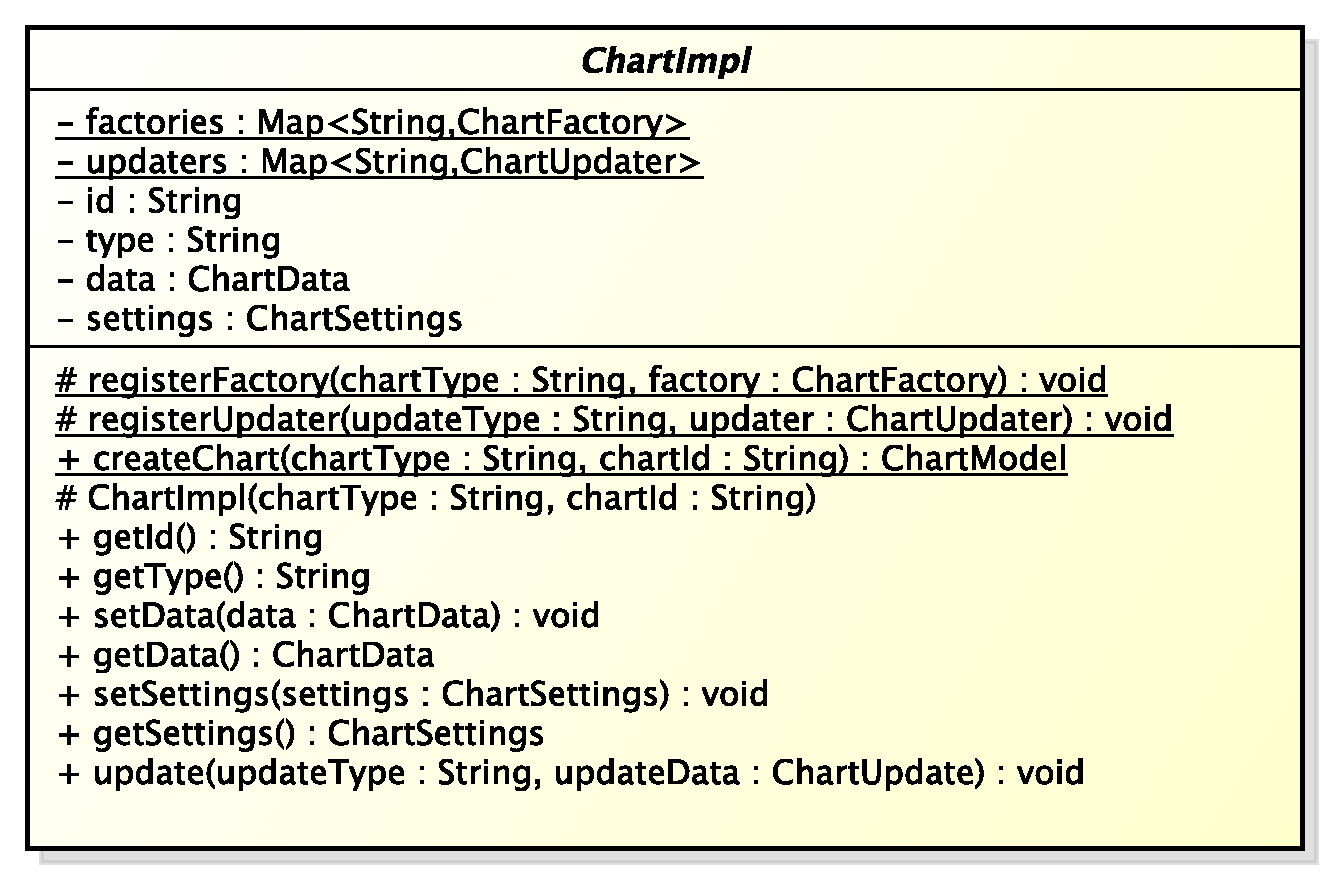
\includegraphics[scale=0.5]{DefinizioneDiProdotto/Pics/Classi/Applicazione--Model--NorrisChart--ChartImpl}
				\caption{Applicazione::Model::NorrisChart::ChartImpl}
			\end{figure}
		}
	
			
			\begin{itemize}
			\item \textbf{Nome:} ChartImpl
			\item \textbf{Tipo:} classe
			
		\item \textbf{Implementa:}
		ChartActivity, ChartModel
		\item \textbf{Astratta:}
		si
			\item \textbf{Visibilità:} public
			\item \textbf{Descrizione:} Questa classe rappresenta un grafico generico e per questo motivo è una classe astratta. Essa contiene al suo interno i dati (ChartData) e le impostazioni (ChartSettings) relativi ad un grafico. Contiene, inoltre, l'interfaccia ChartFactory e due hashmap: la prima si occupa della corrispondenza tra le tipologie di grafico e le rispettive classi factory, la seconda invece si occupa della corrispondenza tra le varie tipologie di aggiornamento e la classe che implementa tale aggiornamento per un tipo specifico di grafico. ChartImpl ha una dipendenza verso l'interfaccia ChartUpdate, in quanto deve conoscere il tipo del pacchetto degli aggiornamenti. 
			\item \textbf{Attributi:}
				\begin{itemize}
				\setlength{\itemsep}{5pt}
				
					\item[\ding{111}] \underline{--factories : Map<String,ChartFactory>} \\ [1mm] Tale hashmap contiene le associazioni di tutti i tipi di chart possibili con la relativa factory del chart.
					\item[\ding{111}] \underline{--updaters : Map<String,ChartUpdater>} \\ [1mm] Tale hashmap contiene le associazioni di tutti gli aggiornamenti possibilli con l'oggetto ChartUpdater.
					\item[\ding{111}] {--id : String} \\ [1mm] Tale attributo rappresenta l'id del chart.
					\item[\ding{111}] {--type : String} \\ [1mm] Tale attributo rappresenta il tipo del chart.
					\item[\ding{111}] {--data : ChartData} \\ [1mm] Tale attributo rappresenta i valori del chart.
					\item[\ding{111}] {--settings : ChartSettings} \\ [1mm] Tale attributo rappresenta le impostazioni del chart.
				\end{itemize}
		
			\item \textbf{Metodi:}
				\begin{itemize}
				\setlength{\itemsep}{5pt}
				
					\item[\ding{111}] {\underline{+create(type : String, id : String) : ChartModel}} \\ [1mm] Tale metodo non fa altro che creare il chart associato al parametro type e ritornare l'interfaccia ChartModel di tale istanza creata. Esso non fa altro che invocare il metodo chreateChart dela classe factory pesente nell'hash map factories con la chiave eguale al parametro type e ne ritornerà tale oggetto creato.
					\item[\ding{111}] {\underline{\#registerFactory(chartType : String, factory : ChartFactory) : void}} \\ [1mm] Tale metodo serve per registrare una certa factory al relativo chart nell'hashmap della classe (factories). Tale metodo viene chiamato dalle classi factory interne ai vari ChartImpl con lo scopo di registrarsi come creatori di chart e poter quindi esser utilizzate per tale scopo.
					\item[\ding{111}] {\underline{\#registerUpdater(updateType : String, updater : ChartUpdater) : void}} \\ [1mm] Tale metodo serve per registrare un certo updater al relativo tipo di update nell'hashmap della classe (updaters). Tale metodo viene invocato dalle classi Updater al loro caricamento per aggiungersi come updater.
					\item[\ding{111}] {{\#ChartImpl(charttype : String, chartid : String)}} \\ [1mm] Tale metodo è il costuttore della classe. Esso è accessibile solamente alle sottoclassi nella creazione del sottoggetto.
					\item[\ding{111}] {{+getData() : ChartData}} \\ [1mm] Tale metodo ha il compito di ritornare i dati del chart.
					\item[\ding{111}] {{+getId() : String}} \\ [1mm] Tale metodo ha il compito di ritornare l'id del chart.
					\item[\ding{111}] {{+getSettings() : ChartSettings}} \\ [1mm] Tale metodo ha il compito di ritornare le impostazioni del chart.
					\item[\ding{111}] {{+getType() : String}} \\ [1mm] Tale metodo ha il compito di ritornare il tipo del chart.
					\item[\ding{111}] {{+setData(data : ChartData) : void}} \\ [1mm] Tale metodo ha il compito di impostare i dati del chart.
					\item[\ding{111}] {{+setSettings(settings : ChartSettings) : void}} \\ [1mm] Tale metodo ha il compito di assegnare le impostazioni del chart.
					\item[\ding{111}] {{+update(updateType : String, updateData : ChartUpdate) : void}} \\ [1mm] Tale metodo ha il compito di aggiornare i chart utilizzando la tipologia di aggiornamento presente in updateType e il pacchetto di aggiornamento updateData. Esso non fa altro che invocare il metodo update dell'updater pesente nell'hash map updaters con la chiave eguale al parametro updateType e passargli come parametro il parametro ricevuto updateData ed  i dati del chart che verranno modificati per riferimento.
				\end{itemize}
		
			\end{itemize}

			
			\level{5}[ChartFactory]{Applicazione::Model::NorrisChart::ChartImpl::ChartFactory}
			

		\IfFileExists{DefinizioneDiProdotto/Pics/Classi/Applicazione--Model--NorrisChart--ChartImpl--ChartFactory.pdf}{
			\begin{figure}[H]
				\centering
				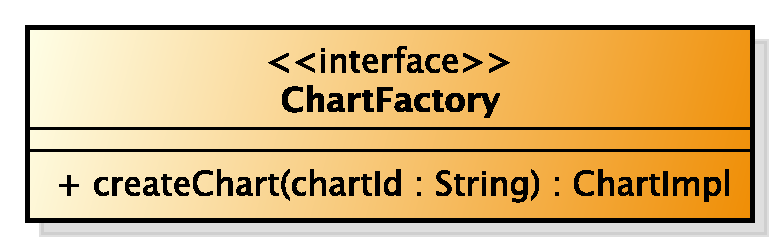
\includegraphics[scale=0.5]{DefinizioneDiProdotto/Pics/Classi/Applicazione--Model--NorrisChart--ChartImpl--ChartFactory}
				\caption{Applicazione::Model::NorrisChart::ChartImpl::ChartFactory}
			\end{figure}
		}
	
			
			\begin{itemize}
			\item \textbf{Nome:} ChartFactory
			\item \textbf{Tipo:} interfaccia
			
			\item \textbf{Visibilità:} protected
			\item \textbf{Descrizione:} ChartFactory è l'interfaccia delle classi factory che si occupano della creazione dei vari tipi di grafici. È interna alla classe ChartImpl.
			\item \textbf{Metodi:}
				\begin{itemize}
				\setlength{\itemsep}{5pt}
				
					\item[\ding{111}] {{+createChart(chartId : String) : ChartImpl}} \\ [1mm] Tale metodo ha il compito di creare la relativa specializzazione di ChartImpl. Esso può accedere al suo costruttore perchè questa classe factory è interna alla relativa classe MapChartImpl.
				\end{itemize}
		
			\end{itemize}

			
			\level{5}[ChartModel]{Applicazione::Model::NorrisChart::ChartModel}
			

		\IfFileExists{DefinizioneDiProdotto/Pics/Classi/Applicazione--Model--NorrisChart--ChartModel.pdf}{
			\begin{figure}[H]
				\centering
				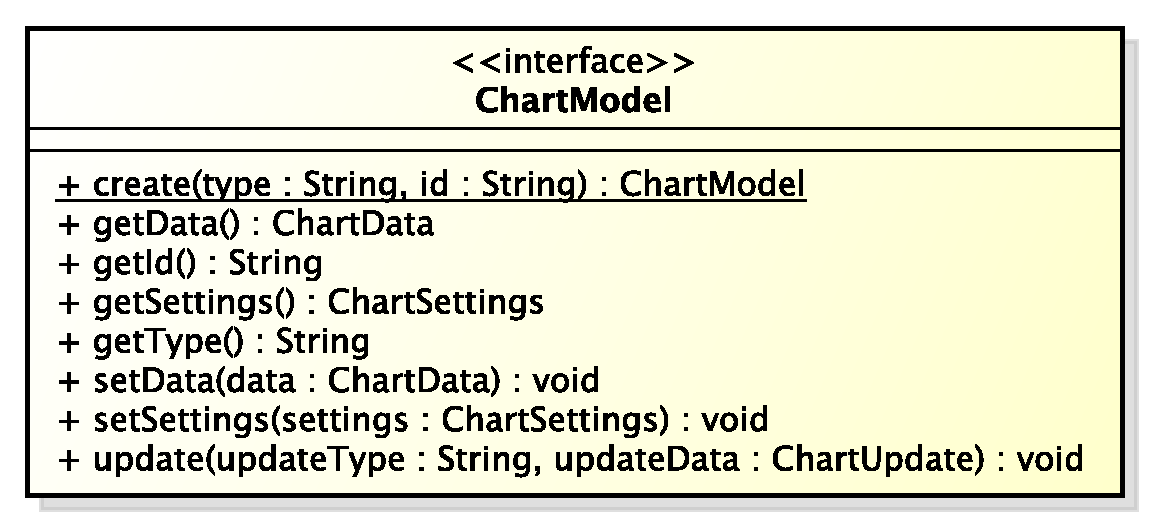
\includegraphics[scale=0.5]{DefinizioneDiProdotto/Pics/Classi/Applicazione--Model--NorrisChart--ChartModel}
				\caption{Applicazione::Model::NorrisChart::ChartModel}
			\end{figure}
		}
	
			
			\begin{itemize}
			\item \textbf{Nome:} ChartModel
			\item \textbf{Tipo:} interfaccia
			
			\item \textbf{Visibilità:} public
			\item \textbf{Descrizione:} Chart è l'interfaccia che rappresenta un grafico generico e viene implementata da ChartImpl. Essa contiene i metodi set e get relativi alle impostazioni e ai dati ed i metodi relativi agli aggiornamenti dei grafici.
			\item \textbf{Metodi:}
				\begin{itemize}
				\setlength{\itemsep}{5pt}
				
					\item[\ding{111}] {{+getData() : ChartData}} \\ [1mm] Tale metodo ha il compito di ritornare i dati del chart.
					\item[\ding{111}] {{+getId() : String}} \\ [1mm] Tale metodo ha il compito di ritornare l'id del chart.
					\item[\ding{111}] {{+getSettings() : ChartSettings}} \\ [1mm] Tale metodo ha il compito di ritornare le impostazioni del chart.
					\item[\ding{111}] {{+getType() : String}} \\ [1mm] Tale metodo ha il compito di ritornare il tipo del chart.
					\item[\ding{111}] {{+setData(data : ChartData) : void}} \\ [1mm] Tale metodo ha il compito di impostare i dati del chart.
					\item[\ding{111}] {{+setSettings(settings : ChartSettings) : void}} \\ [1mm] Tale metodo ha il compito di assegnare le impostazioni del chart.
					\item[\ding{111}] {{+update(updateType : String, updateData : ChartUpdate) : void}} \\ [1mm] Tale metodo ha il compito di aggiornare i chart utilizzando la tipologia di aggiornamento presente in updateType e il pacchetto di aggiornamento updateData.
				\end{itemize}
		
			\end{itemize}

			
			\level{5}[ChartSettings]{Applicazione::Model::NorrisChart::ChartSettings}
			

		\IfFileExists{DefinizioneDiProdotto/Pics/Classi/Applicazione--Model--NorrisChart--ChartSettings.pdf}{
			\begin{figure}[H]
				\centering
				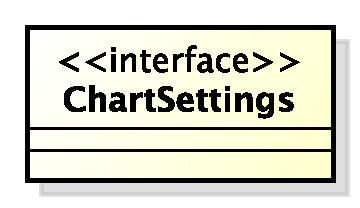
\includegraphics[scale=0.5]{DefinizioneDiProdotto/Pics/Classi/Applicazione--Model--NorrisChart--ChartSettings}
				\caption{Applicazione::Model::NorrisChart::ChartSettings}
			\end{figure}
		}
	
			
			\begin{itemize}
			\item \textbf{Nome:} ChartSettings
			\item \textbf{Tipo:} interfaccia
			
			\item \textbf{Visibilità:} public
			\item \textbf{Descrizione:} ChartSettings è l'interfaccia delle classi che si occupano delle impostazioni di un grafico. 
			\end{itemize}

			
			\level{5}[ChartUpdate]{Applicazione::Model::NorrisChart::ChartUpdate}
			

		\IfFileExists{DefinizioneDiProdotto/Pics/Classi/Applicazione--Model--NorrisChart--ChartUpdate.pdf}{
			\begin{figure}[H]
				\centering
				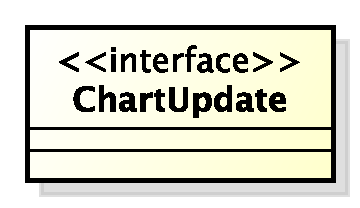
\includegraphics[scale=0.5]{DefinizioneDiProdotto/Pics/Classi/Applicazione--Model--NorrisChart--ChartUpdate}
				\caption{Applicazione::Model::NorrisChart::ChartUpdate}
			\end{figure}
		}
	
			
			\begin{itemize}
			\item \textbf{Nome:} ChartUpdate
			\item \textbf{Tipo:} interfaccia
			
			\item \textbf{Visibilità:} public
			\item \textbf{Descrizione:} ChartUpdate è l'interfaccia delle classi che si occupano dell'aggiornamento di un grafico. In particolare rappresenta il pacchetto di aggiornamento di un grafico.
			\end{itemize}

			
			\level{5}[ChartUpdater]{Applicazione::Model::NorrisChart::ChartUpdater}
			

		\IfFileExists{DefinizioneDiProdotto/Pics/Classi/Applicazione--Model--NorrisChart--ChartUpdater.pdf}{
			\begin{figure}[H]
				\centering
				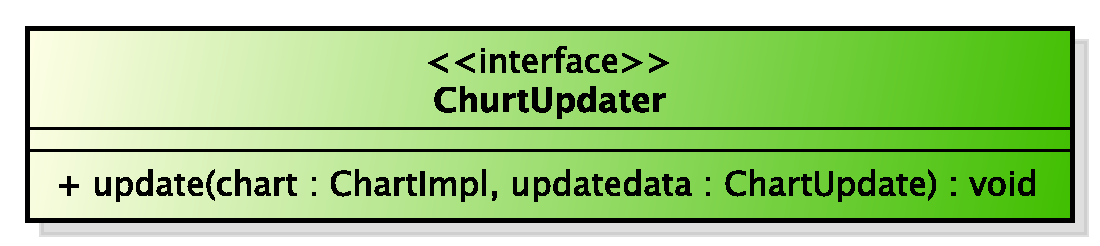
\includegraphics[scale=0.5]{DefinizioneDiProdotto/Pics/Classi/Applicazione--Model--NorrisChart--ChartUpdater}
				\caption{Applicazione::Model::NorrisChart::ChartUpdater}
			\end{figure}
		}
	
			
			\begin{itemize}
			\item \textbf{Nome:} ChartUpdater
			\item \textbf{Tipo:} interfaccia
			
			\item \textbf{Visibilità:} protected
			\item \textbf{Descrizione:} Updater è l'interfaccia delle classi che si occupano dell'implementazione dei vari tipi di aggiornamento per ogni tipologia di grafico.
			\item \textbf{Metodi:}
				\begin{itemize}
				\setlength{\itemsep}{5pt}
				
					\item[\ding{111}] {{+update(chart : ChartImpl, updateData : ChartUpdate) : void}} \\ [1mm] Tale metodo ha il compito di aggiornare il chart passato come parametro (chart) utilizzando il pacchetto di aggiornamento (updatedata).
				\end{itemize}
		
			\end{itemize}

			
			\level{5}[LineChartImpl]{Applicazione::Model::NorrisChart::LineChartImpl}
			

		\IfFileExists{DefinizioneDiProdotto/Pics/Classi/Applicazione--Model--NorrisChart--LineChartImpl.pdf}{
			\begin{figure}[H]
				\centering
				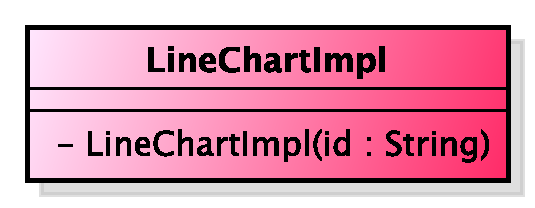
\includegraphics[scale=0.5]{DefinizioneDiProdotto/Pics/Classi/Applicazione--Model--NorrisChart--LineChartImpl}
				\caption{Applicazione::Model::NorrisChart::LineChartImpl}
			\end{figure}
		}
	
			
			\begin{itemize}
			\item \textbf{Nome:} LineChartImpl
			\item \textbf{Tipo:} classe
			
		\item \textbf{Estende:}
		ChartImpl
		\item \textbf{Astratta:}
		no
			\item \textbf{Visibilità:} package
			\item \textbf{Descrizione:} Questa classe rappresenta un grafico di tipo line chart. Essa contiene al suo interno i dati (LineChartDataObject) e le impostazioni (LineChartSettingsObject) relativi al grafico. Inoltre contiene le classi LineChartInPlaceUpdater e LineChartStreamUpdater, le quali implementano rispettivamente l'aggiornamento di tipo in place e stream per il grafico in questione. Un'istanza della classe LineChartImpl viene creata dalla classe factory LineChartFactory.
			\item \textbf{Metodi:}
				\begin{itemize}
				\setlength{\itemsep}{5pt}
				
					\item[\ding{111}] {{--LineChartImpl(chartId : String)}} \\ [1mm] Tale metodo è il costruttore. Esso è privato perchè non può esser creata una istanza se non dalla sua classe interna factory.
				\end{itemize}
		
			\end{itemize}

			
			\level{5}[LineChartFactory]{Applicazione::Model::NorrisChart::LineChartImpl::LineChartFactory}
			

		\IfFileExists{DefinizioneDiProdotto/Pics/Classi/Applicazione--Model--NorrisChart--LineChartImpl--LineChartFactory.pdf}{
			\begin{figure}[H]
				\centering
				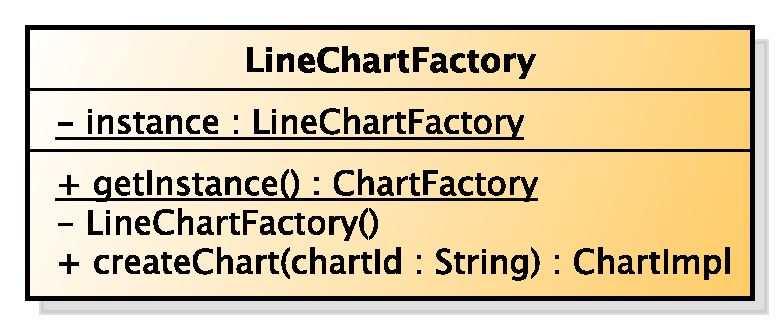
\includegraphics[scale=0.5]{DefinizioneDiProdotto/Pics/Classi/Applicazione--Model--NorrisChart--LineChartImpl--LineChartFactory}
				\caption{Applicazione::Model::NorrisChart::LineChartImpl::LineChartFactory}
			\end{figure}
		}
	
			
			\begin{itemize}
			\item \textbf{Nome:} LineChartFactory
			\item \textbf{Tipo:} classe
			
		\item \textbf{Implementa:}
		ChartFactory
		\item \textbf{Astratta:}
		no
			\item \textbf{Visibilità:} private
			\item \textbf{Descrizione:} Questa classe si occupa della creazione di un grafico di tipo LineChartImpl. In particolare si occupa di configurare i dati e le impostazioni del grafico. Tale classe dispone di un blocco di inizializzazione statica che registra la sua istanza nel HashMap factories della classe ChartImpl non appena tale classe viene caricata.
			\item \textbf{Attributi:}
				\begin{itemize}
				\setlength{\itemsep}{5pt}
				
					\item[\ding{111}] \underline{--instance : LineChartFactory} \\ [1mm] Tale attributo statico rappresenta l'istanza univoca di tale classe.
				\end{itemize}
		
			\item \textbf{Metodi:}
				\begin{itemize}
				\setlength{\itemsep}{5pt}
				
					\item[\ding{111}] {\underline{+getInstance() : ChartFactory}} \\ [1mm] Tale metodo ha il compito di ritornare l'istanza unica di tale classe e se non esiste la crea.
					\item[\ding{111}] {{--LineChartFactory()}} \\ [1mm] Tale metodo è il costruttore della classe. Esso è privato perchè non si vuole permettere a nessuno di poter creare un'istanza se non utilizzando il metodo getInstance().
					\item[\ding{111}] {{+createChart(chartId : String) : ChartImpl}} \\ [1mm] Tale metodo ha il compito di creare la relativa specializzazione di ChartImpl. Esso può accedere al suo costruttore perchè questa classe factory è interna alla relativa classe LineChartImpl.
				\end{itemize}
		
			\end{itemize}

			
			\level{5}[LineChartInPlaceUpdater]{Applicazione::Model::NorrisChart::LineChartInPlaceUpdater}
			

		\IfFileExists{DefinizioneDiProdotto/Pics/Classi/Applicazione--Model--NorrisChart--LineChartInPlaceUpdater.pdf}{
			\begin{figure}[H]
				\centering
				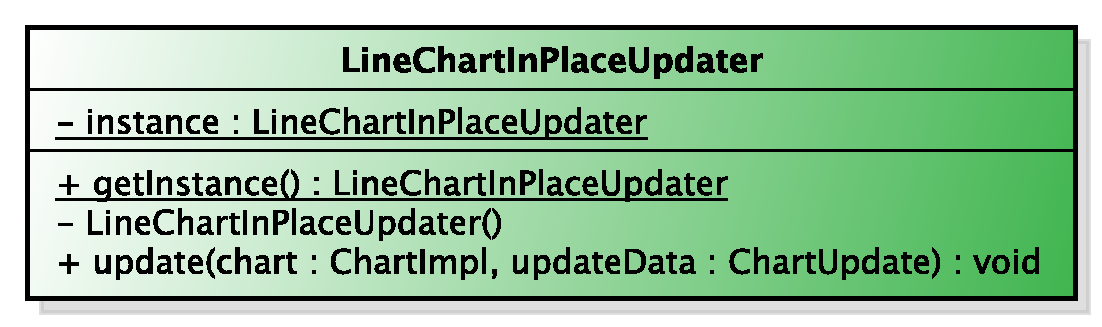
\includegraphics[scale=0.5]{DefinizioneDiProdotto/Pics/Classi/Applicazione--Model--NorrisChart--LineChartInPlaceUpdater}
				\caption{Applicazione::Model::NorrisChart::LineChartInPlaceUpdater}
			\end{figure}
		}
	
			
			\begin{itemize}
			\item \textbf{Nome:} LineChartInPlaceUpdater
			\item \textbf{Tipo:} classe
			
		\item \textbf{Implementa:}
		ChartUpdater
		\item \textbf{Astratta:}
		no
			\item \textbf{Visibilità:} package
			\item \textbf{Descrizione:} Questa classe si occupa di definire il metodo di aggiornamento in place per un grafico di tipo line chart. Essendo una classe interna di LineChartImpl, ha acceso ai campi dati privati di questa classe. In particolare può accedere al DataObject contenuto in LineChartImpl e modificarne i valori.
			\item \textbf{Attributi:}
				\begin{itemize}
				\setlength{\itemsep}{5pt}
				
					\item[\ding{111}] \underline{--instance : LineChartInPlaceUpdater} \\ [1mm] Tale attributo statico rappresenta l'istanza univoca di tale classe.
				\end{itemize}
		
			\item \textbf{Metodi:}
				\begin{itemize}
				\setlength{\itemsep}{5pt}
				
					\item[\ding{111}] {\underline{+getInstance() : ChartUpdater}} \\ [1mm] Tale metodo ha il compito di ritornare l'istanza unica di tale classe e se non esiste la crea.
					\item[\ding{111}] {{+update(chart : ChartImpl, updateData : ChartUpdate) : void}} \\ [1mm] Tale metodo ha il compito di aggiornare il chart passato come parametro (chart) utilizzando il pacchetto di aggiornamento (updatedata).
				\end{itemize}
		
			\end{itemize}

			
			\level{5}[LineChartStreaUpdater]{Applicazione::Model::NorrisChart::LineChartStreaUpdater}
			

		\IfFileExists{DefinizioneDiProdotto/Pics/Classi/Applicazione--Model--NorrisChart--LineChartStreaUpdater.pdf}{
			\begin{figure}[H]
				\centering
				\includegraphics[scale=0.5]{DefinizioneDiProdotto/Pics/Classi/Applicazione--Model--NorrisChart--LineChartStreaUpdater}
				\caption{Applicazione::Model::NorrisChart::LineChartStreaUpdater}
			\end{figure}
		}
	
			
			\begin{itemize}
			\item \textbf{Nome:} LineChartStreaUpdater
			\item \textbf{Tipo:} classe
			
		\item \textbf{Implementa:}
		ChartUpdater
		\item \textbf{Astratta:}
		no
			\item \textbf{Visibilità:} package
			\item \textbf{Descrizione:} Questa classe si occupa di definire il metodo di aggiornamento stream per un grafico di tipo line chart. Essendo una classe interna di LineChartImpl, ha acceso ai campi dati privati di questa classe. In particolare può accedere al DataObject contenuto in LineChartImpl e modificarne i valori.
			\item \textbf{Attributi:}
				\begin{itemize}
				\setlength{\itemsep}{5pt}
				
					\item[\ding{111}] \underline{--instance : LineChartStreaUpdater} \\ [1mm] Tale attributo statico rappresenta l'istanza univoca di tale classe.
				\end{itemize}
		
			\item \textbf{Metodi:}
				\begin{itemize}
				\setlength{\itemsep}{5pt}
				
					\item[\ding{111}] {\underline{+getInstance() : ChartUpdater}} \\ [1mm] Tale metodo ha il compito di ritornare l'istanza unica di tale classe e se non esiste la crea.
					\item[\ding{111}] {{+update(chart : ChartImpl, updateData : ChartUpdate) : void}} \\ [1mm] Tale metodo ha il compito di aggiornare il chart passato come parametro (chart) utilizzando il pacchetto di aggiornamento (updatedata).
				\end{itemize}
		
			\end{itemize}

			
			\level{5}[MapChartImpl]{Applicazione::Model::NorrisChart::MapChartImpl}
			

		\IfFileExists{DefinizioneDiProdotto/Pics/Classi/Applicazione--Model--NorrisChart--MapChartImpl.pdf}{
			\begin{figure}[H]
				\centering
				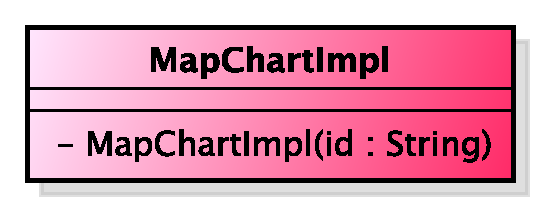
\includegraphics[scale=0.5]{DefinizioneDiProdotto/Pics/Classi/Applicazione--Model--NorrisChart--MapChartImpl}
				\caption{Applicazione::Model::NorrisChart::MapChartImpl}
			\end{figure}
		}
	
			
			\begin{itemize}
			\item \textbf{Nome:} MapChartImpl
			\item \textbf{Tipo:} classe
			
		\item \textbf{Estende:}
		ChartImpl
		\item \textbf{Astratta:}
		no
			\item \textbf{Visibilità:} package
			\item \textbf{Descrizione:} Questa classe rappresenta un grafico di tipo map chart. Essa contiene al suo interno i dati (MapChartDataObject) e le impostazioni (MapChartSettingsObject) relativi al grafico. Inoltre contiene le classi MapChartInPlaceUpdater e MapChartMovieUpdater, le quali implementano rispettivamente l'aggiornamento di tipo in place e movie per il grafico in questione. Un'istanza della classe MapChartImpl viene creata dalla classe factory MapChartFactory.
			\item \textbf{Metodi:}
				\begin{itemize}
				\setlength{\itemsep}{5pt}
				
					\item[\ding{111}] {{--MapChartImpl(chartId : String)}} \\ [1mm] Tale metodo è il costruttore. Esso è privato perchè non può esser creata una istanza se non dalla sua classe interna factory.
				\end{itemize}
		
			\end{itemize}

			
			\level{5}[MapChartFactory]{Applicazione::Model::NorrisChart::MapChartImpl::MapChartFactory}
			

		\IfFileExists{DefinizioneDiProdotto/Pics/Classi/Applicazione--Model--NorrisChart--MapChartImpl--MapChartFactory.pdf}{
			\begin{figure}[H]
				\centering
				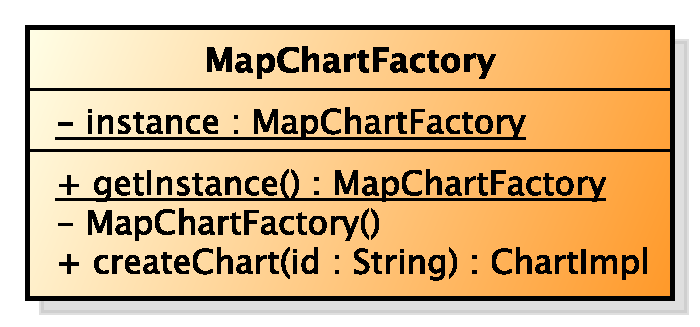
\includegraphics[scale=0.5]{DefinizioneDiProdotto/Pics/Classi/Applicazione--Model--NorrisChart--MapChartImpl--MapChartFactory}
				\caption{Applicazione::Model::NorrisChart::MapChartImpl::MapChartFactory}
			\end{figure}
		}
	
			
			\begin{itemize}
			\item \textbf{Nome:} MapChartFactory
			\item \textbf{Tipo:} classe
			
		\item \textbf{Implementa:}
		ChartFactory
		\item \textbf{Astratta:}
		no
			\item \textbf{Visibilità:} private
			\item \textbf{Descrizione:} Questa classe si occupa della creazione di un grafico di tipo MapChartImpl. In particolare si occupa di configurare i dati e le impostazioni del grafico. Tale classe dispone di un blocco di inizializzazione statica che registra la sua istanza nel HashMap factories della classe ChartImpl non appena tale classe viene caricata.
			\item \textbf{Attributi:}
				\begin{itemize}
				\setlength{\itemsep}{5pt}
				
					\item[\ding{111}] \underline{--instance : MapChartFactory} \\ [1mm] Tale attributo statico rappresenta l'istanza univoca di tale classe.
				\end{itemize}
		
			\item \textbf{Metodi:}
				\begin{itemize}
				\setlength{\itemsep}{5pt}
				
					\item[\ding{111}] {\underline{+getInstance() : ChartFactory}} \\ [1mm] Tale metodo ha il compito di ritornare l'istanza unica di tale classe e se non esiste la crea.
					\item[\ding{111}] {{--MapChartFactory()}} \\ [1mm] Tale metodo è il costruttore della classe. Esso è privato perchè non si vuole permettere a nessuno di poter creare un'istanza se non utilizzando il metodo getInstance().
					\item[\ding{111}] {{+createChart(chartId : String) : ChartImpl}} \\ [1mm] Tale metodo ha il compito di creare la relativa specializzazione di ChartImpl. Esso può accedere al suo costruttore perchè questa classe factory è interna alla relativa classe MapChartImpl.
				\end{itemize}
		
			\end{itemize}

			
			\level{5}[MapChartInPlaceUpdater]{Applicazione::Model::NorrisChart::MapChartInPlaceUpdater}
			

		\IfFileExists{DefinizioneDiProdotto/Pics/Classi/Applicazione--Model--NorrisChart--MapChartInPlaceUpdater.pdf}{
			\begin{figure}[H]
				\centering
				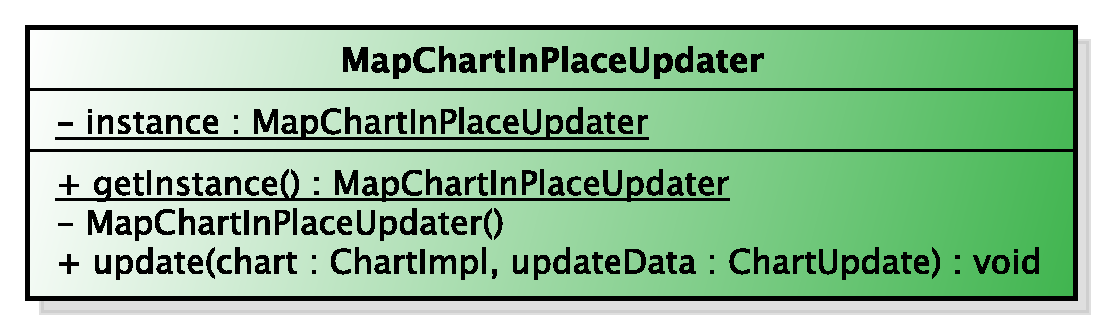
\includegraphics[scale=0.5]{DefinizioneDiProdotto/Pics/Classi/Applicazione--Model--NorrisChart--MapChartInPlaceUpdater}
				\caption{Applicazione::Model::NorrisChart::MapChartInPlaceUpdater}
			\end{figure}
		}
	
			
			\begin{itemize}
			\item \textbf{Nome:} MapChartInPlaceUpdater
			\item \textbf{Tipo:} classe
			
		\item \textbf{Implementa:}
		ChartUpdater
		\item \textbf{Astratta:}
		no
			\item \textbf{Visibilità:} package
			\item \textbf{Descrizione:} Questa classe si occupa di definire il metodo di aggiornamento in place per un grafico di tipo map chart. Essendo una classe interna di MapChartImpl, ha acceso ai campi dati privati di questa classe. In particolare può accedere al DataObject contenuto in MapChartImpl e modificarne i valori.
			\item \textbf{Attributi:}
				\begin{itemize}
				\setlength{\itemsep}{5pt}
				
					\item[\ding{111}] \underline{--instance : MapChartInPlaceUpdater} \\ [1mm] Tale attributo statico rappresenta l'istanza univoca di tale classe.
				\end{itemize}
		
			\item \textbf{Metodi:}
				\begin{itemize}
				\setlength{\itemsep}{5pt}
				
					\item[\ding{111}] {\underline{+getInstance() : ChartUpdater}} \\ [1mm] Tale metodo ha il compito di ritornare l'istanza unica di tale classe e se non esiste la crea.
					\item[\ding{111}] {{+update(chart : ChartImpl, updateData : ChartUpdate) : void}} \\ [1mm] Tale metodo ha il compito di aggiornare il chart passato come parametro (chart) utilizzando il pacchetto di aggiornamento (updatedata).
				\end{itemize}
		
			\end{itemize}

			
			\level{5}[MapChartMovieUpdater]{Applicazione::Model::NorrisChart::MapChartMovieUpdater}
			

		\IfFileExists{DefinizioneDiProdotto/Pics/Classi/Applicazione--Model--NorrisChart--MapChartMovieUpdater.pdf}{
			\begin{figure}[H]
				\centering
				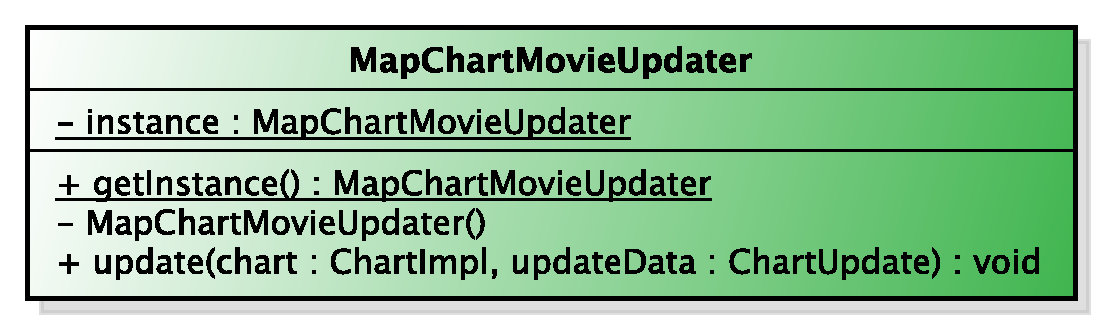
\includegraphics[scale=0.5]{DefinizioneDiProdotto/Pics/Classi/Applicazione--Model--NorrisChart--MapChartMovieUpdater}
				\caption{Applicazione::Model::NorrisChart::MapChartMovieUpdater}
			\end{figure}
		}
	
			
			\begin{itemize}
			\item \textbf{Nome:} MapChartMovieUpdater
			\item \textbf{Tipo:} classe
			
		\item \textbf{Implementa:}
		ChartUpdater
		\item \textbf{Astratta:}
		no
			\item \textbf{Visibilità:} package
			\item \textbf{Descrizione:} Questa classe si occupa di definire il metodo di aggiornamento movie per un grafico di tipo map chart. Essendo una classe interna di MapChartImpl, ha acceso ai campi dati privati di questa classe. In particolare può accedere al DataObject contenuto in MapChartImpl e modificarne i valori.
			\item \textbf{Attributi:}
				\begin{itemize}
				\setlength{\itemsep}{5pt}
				
					\item[\ding{111}] \underline{--instance : MapChartMovieUpdater} \\ [1mm] Tale attributo statico rappresenta l'istanza univoca di tale classe.
				\end{itemize}
		
			\item \textbf{Metodi:}
				\begin{itemize}
				\setlength{\itemsep}{5pt}
				
					\item[\ding{111}] {\underline{+getInstance() : ChartUpdater}} \\ [1mm] Tale metodo ha il compito di ritornare l'istanza unica di tale classe e se non esiste la crea.
					\item[\ding{111}] {{+update(chart : ChartImpl, updateData : ChartUpdate) : void}} \\ [1mm] Tale metodo ha il compito di aggiornare il chart passato come parametro (chart) utilizzando il pacchetto di aggiornamento (updatedata).
				\end{itemize}
		
			\end{itemize}

			
			\level{5}[TableImpl]{Applicazione::Model::NorrisChart::TableImpl}
			

		\IfFileExists{DefinizioneDiProdotto/Pics/Classi/Applicazione--Model--NorrisChart--TableImpl.pdf}{
			\begin{figure}[H]
				\centering
				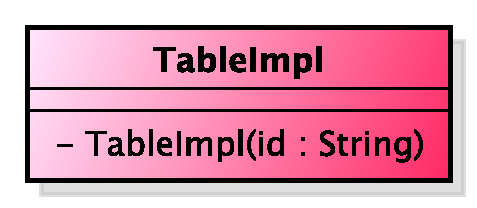
\includegraphics[scale=0.5]{DefinizioneDiProdotto/Pics/Classi/Applicazione--Model--NorrisChart--TableImpl}
				\caption{Applicazione::Model::NorrisChart::TableImpl}
			\end{figure}
		}
	
			
			\begin{itemize}
			\item \textbf{Nome:} TableImpl
			\item \textbf{Tipo:} classe
			
		\item \textbf{Estende:}
		ChartImpl
		\item \textbf{Astratta:}
		no
			\item \textbf{Visibilità:} package
			\item \textbf{Descrizione:} Questa classe rappresenta un grafico di tipo table. Essa contiene al suo interno i dati (TableDataObject) e le impostazioni (TableSettingsObject) relativi al grafico. Inoltre contiene le classi TableInPlaceUpdater e TableStreamUpdater, le quali implementano rispettivamente l'aggiornamento di tipo in place e stream per il grafico in questione. Un'istanza della classe TableImpl viene creata dalla classe factory TableFactory.
			\item \textbf{Metodi:}
				\begin{itemize}
				\setlength{\itemsep}{5pt}
				
					\item[\ding{111}] {{--TableImpl(chartId : String)}} \\ [1mm] Tale metodo è il costruttore. Esso è privato perchè non può esser creata una istanza se non dalla sua classe interna factory.
				\end{itemize}
		
			\end{itemize}

			
			\level{5}[TableFactory]{Applicazione::Model::NorrisChart::TableImpl::TableFactory}
			

		\IfFileExists{DefinizioneDiProdotto/Pics/Classi/Applicazione--Model--NorrisChart--TableImpl--TableFactory.pdf}{
			\begin{figure}[H]
				\centering
				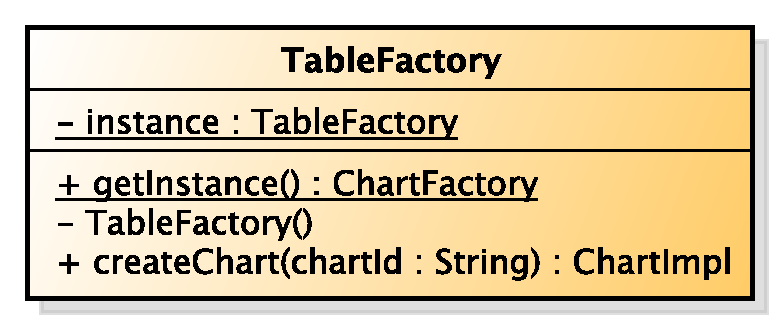
\includegraphics[scale=0.5]{DefinizioneDiProdotto/Pics/Classi/Applicazione--Model--NorrisChart--TableImpl--TableFactory}
				\caption{Applicazione::Model::NorrisChart::TableImpl::TableFactory}
			\end{figure}
		}
	
			
			\begin{itemize}
			\item \textbf{Nome:} TableFactory
			\item \textbf{Tipo:} classe
			
		\item \textbf{Implementa:}
		ChartFactory
		\item \textbf{Astratta:}
		no
			\item \textbf{Visibilità:} private
			\item \textbf{Descrizione:} Questa classe si occupa della creazione di un grafico di tipo TableImpl. Tale classe dispone di un blocco di inizializzazione statica che registra la sua istanza nel HashMap factories della classe ChartImpl non appena tale classe viene caricata.
			\item \textbf{Attributi:}
				\begin{itemize}
				\setlength{\itemsep}{5pt}
				
					\item[\ding{111}] \underline{--instance : TableFactory} \\ [1mm] Tale attributo statico rappresenta l'istanza univoca di tale classe.
				\end{itemize}
		
			\item \textbf{Metodi:}
				\begin{itemize}
				\setlength{\itemsep}{5pt}
				
					\item[\ding{111}] {\underline{+getInstance() : ChartFactory}} \\ [1mm] Tale metodo ha il compito di ritornare l'istanza unica di tale classe e se non esiste la crea.
					\item[\ding{111}] {{--TableFactory()}} \\ [1mm] Tale metodo è il costruttore della classe. Esso è privato perchè non si vuole permettere a nessuno di poter creare un'istanza se non utilizzando il metodo getInstance().
					\item[\ding{111}] {{+createChart(chartId : String) : ChartImpl}} \\ [1mm] Tale metodo ha il compito di creare la relativa specializzazione di ChartImpl. Esso può accedere al suo costruttore perchè questa classe factory è interna alla relativa classe TableImpl
				\end{itemize}
		
			\end{itemize}

			
			\level{5}[TableInPlaceUpdater]{Applicazione::Model::NorrisChart::TableInPlaceUpdater}
			

		\IfFileExists{DefinizioneDiProdotto/Pics/Classi/Applicazione--Model--NorrisChart--TableInPlaceUpdater.pdf}{
			\begin{figure}[H]
				\centering
				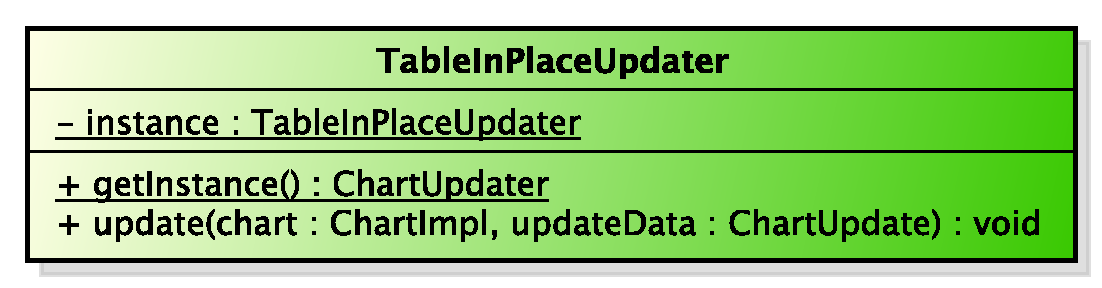
\includegraphics[scale=0.5]{DefinizioneDiProdotto/Pics/Classi/Applicazione--Model--NorrisChart--TableInPlaceUpdater}
				\caption{Applicazione::Model::NorrisChart::TableInPlaceUpdater}
			\end{figure}
		}
	
			
			\begin{itemize}
			\item \textbf{Nome:} TableInPlaceUpdater
			\item \textbf{Tipo:} classe
			
		\item \textbf{Implementa:}
		ChartUpdater
		\item \textbf{Astratta:}
		no
			\item \textbf{Visibilità:} package
			\item \textbf{Descrizione:} Questa classe si occupa di definire il metodo di aggiornamento in place per un grafico di tipo table. Essendo una classe interna di TableImpl, ha acceso ai campi dati privati di questa classe. In particolare può accedere al DataObject contenuto in TableImpl e modificarne i valori.
			\item \textbf{Attributi:}
				\begin{itemize}
				\setlength{\itemsep}{5pt}
				
					\item[\ding{111}] \underline{--instance : TableInPlaceUpdater} \\ [1mm] Tale attributo statico rappresenta l'istanza univoca di tale classe.
				\end{itemize}
		
			\item \textbf{Metodi:}
				\begin{itemize}
				\setlength{\itemsep}{5pt}
				
					\item[\ding{111}] {\underline{+getInstance() : ChartUpdater}} \\ [1mm] Tale metodo ha il compito di ritornare l'istanza unica di tale classe e se non esiste la crea.
					\item[\ding{111}] {{+update(chart : ChartImpl, updateData : ChartUpdate) : void}} \\ [1mm] Tale metodo ha il compito di aggiornare il chart passato come parametro (chart) utilizzando il pacchetto di aggiornamento (updatedata).
				\end{itemize}
		
			\end{itemize}

			
			\level{5}[TableStreamUpdater]{Applicazione::Model::NorrisChart::TableStreamUpdater}
			

		\IfFileExists{DefinizioneDiProdotto/Pics/Classi/Applicazione--Model--NorrisChart--TableStreamUpdater.pdf}{
			\begin{figure}[H]
				\centering
				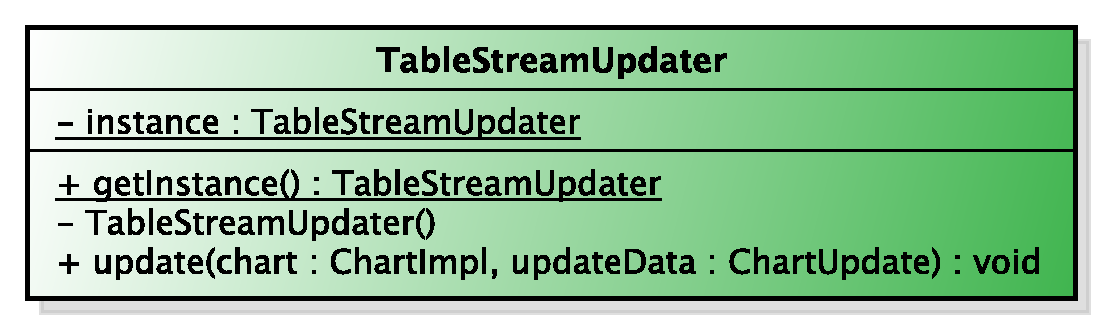
\includegraphics[scale=0.5]{DefinizioneDiProdotto/Pics/Classi/Applicazione--Model--NorrisChart--TableStreamUpdater}
				\caption{Applicazione::Model::NorrisChart::TableStreamUpdater}
			\end{figure}
		}
	
			
			\begin{itemize}
			\item \textbf{Nome:} TableStreamUpdater
			\item \textbf{Tipo:} classe
			
		\item \textbf{Implementa:}
		ChartUpdater
		\item \textbf{Astratta:}
		no
			\item \textbf{Visibilità:} package
			\item \textbf{Descrizione:} Questa classe si occupa di definire il metodo di aggiornamento stream per un grafico di tipo table. Essendo una classe interna di TableImpl, ha acceso ai campi dati privati di questa classe. In particolare può accedere al DataObject contenuto in TableImpl e modificarne i valori.
			\item \textbf{Attributi:}
				\begin{itemize}
				\setlength{\itemsep}{5pt}
				
					\item[\ding{111}] \underline{--instance : TableStreamUpdater} \\ [1mm] Tale attributo statico rappresenta l'istanza univoca di tale classe.
				\end{itemize}
		
			\item \textbf{Metodi:}
				\begin{itemize}
				\setlength{\itemsep}{5pt}
				
					\item[\ding{111}] {\underline{+getInstance() : ChartUpdater}} \\ [1mm] Tale metodo ha il compito di ritornare l'istanza unica di tale classe e se non esiste la crea.
					\item[\ding{111}] {{+update(chart : ChartImpl, updateData : ChartUpdate) : void}} \\ [1mm] Tale metodo ha il compito di aggiornare il chart passato come parametro (chart) utilizzando il pacchetto di aggiornamento (updatedata).
				\end{itemize}
		
			\end{itemize}

			
			\level{5}[NorrisSessionInfo]{Applicazione::Model::NorrisSessionInfo}
			

		\IfFileExists{DefinizioneDiProdotto/Pics/Classi/Applicazione--Model--NorrisSessionInfo.pdf}{
			\begin{figure}[H]
				\centering
				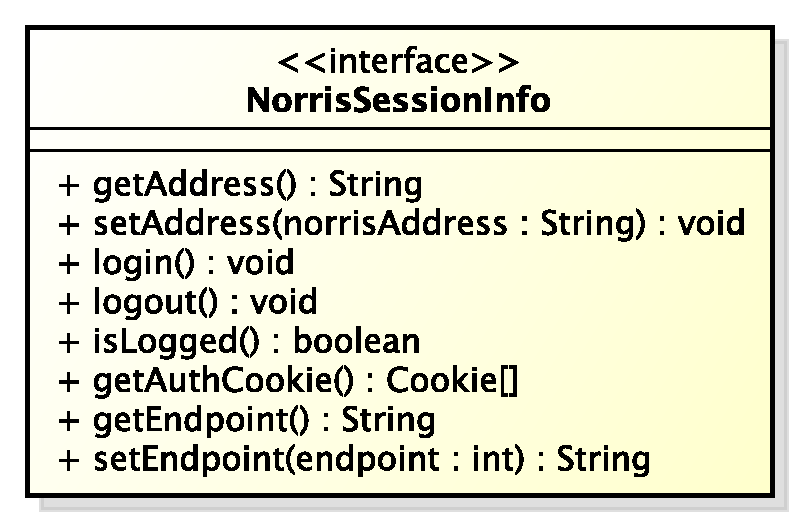
\includegraphics[scale=0.5]{DefinizioneDiProdotto/Pics/Classi/Applicazione--Model--NorrisSessionInfo}
				\caption{Applicazione::Model::NorrisSessionInfo}
			\end{figure}
		}
	
			
			\begin{itemize}
			\item \textbf{Nome:} NorrisSessionInfo
			\item \textbf{Tipo:} interfaccia
			
			\item \textbf{Visibilità:} public
			\item \textbf{Descrizione:} NorrisSessionInfo è l'interfaccia di NorrisSessionInfoImpl.
			\item \textbf{Metodi:}
				\begin{itemize}
				\setlength{\itemsep}{5pt}
				
					\item[\ding{111}] {{+getAddress() : String}} \\ [1mm] Tale metodo ha il compito di ritornare l'indirizzo dell'istanza di Norris.
					\item[\ding{111}] {{+setAddress(norrisAddress : String) : void}} \\ [1mm] Tale metodo ha il compito di memorizzare l'indirizzo dell'istanza di Norris acceduta.
					\item[\ding{111}] {{+login() : void}} \\ [1mm] Tale metodo ha il compito di memorizzare il fatto che è avvenuto il login all'istanza di Norris.
					\item[\ding{111}] {{+logout() : void}} \\ [1mm] Tale metodo ha il compito di memorizzare il fatto che è avvenuto il logout all'istanza di Norris.
					\item[\ding{111}] {{+isLogged() : boolean}} \\ [1mm] Tale metodo ha il compito di informare attraverso una valore booleano se la sessione all'istanza di Norris è attiva.
					\item[\ding{111}] {{+getAuthCookie() : Cookie[]}} \\ [1mm] Tale metodo ha il compito di ritornare l'inieme dei cookie di autenticazione per l'istanza di Norris.
					\item[\ding{111}] {{+getEndpoint() : String}} \\ [1mm] Tale metodo ritorna l'endpoint della sessione corrente. Esso serve per formare i path delle connessioni socket e per formare l'url per le richieste http.
					\item[\ding{111}] {{+setEndpoint(endpoint : int) : String}} \\ [1mm] Tale metodo imposta l'endpoint della sessione corrente. Esso serve per formare i path delle connessioni socket e per formare l'url per le richieste http.
				\end{itemize}
		
			\end{itemize}

			
			\level{5}[NorrisSessionInfoImpl]{Applicazione::Model::NorrisSessionInfoImpl}
			

		\IfFileExists{DefinizioneDiProdotto/Pics/Classi/Applicazione--Model--NorrisSessionInfoImpl.pdf}{
			\begin{figure}[H]
				\centering
				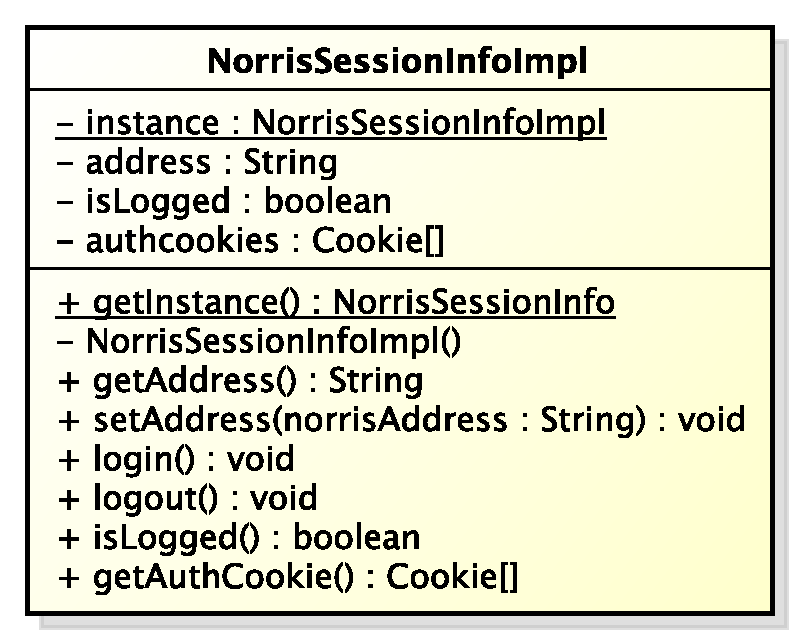
\includegraphics[scale=0.5]{DefinizioneDiProdotto/Pics/Classi/Applicazione--Model--NorrisSessionInfoImpl}
				\caption{Applicazione::Model::NorrisSessionInfoImpl}
			\end{figure}
		}
	
			
			\begin{itemize}
			\item \textbf{Nome:} NorrisSessionInfoImpl
			\item \textbf{Tipo:} classe
			
		\item \textbf{Implementa:}
		NorrisSessionInfo
		\item \textbf{Astratta:}
		no
			\item \textbf{Visibilità:} public
			\item \textbf{Descrizione:} Tale classe ha lo scopo di salvare i vari dati necessari alla sessione. Infatti in essa sono contenuti i vari cookie di autenticazione e l'indirizzo al quale la sessione appartiene.
			\item \textbf{Attributi:}
				\begin{itemize}
				\setlength{\itemsep}{5pt}
				
					\item[\ding{111}] \underline{--instance : NorrisSessionInfoImpl} \\ [1mm] Tale attributo statico rappresenta l'istanza univoca di tale classe.
					\item[\ding{111}] {--address : String} \\ [1mm] Tale attributo rappresenta l'indirizzo di Norris appartenente alla sessione attiva.
					\item[\ding{111}] {--isLogged : boolean} \\ [1mm] Tale attributo rappresenta lo stato della sessione.
					\item[\ding{111}] {--authcookies : Cookie[]} \\ [1mm] Tale attributo rappresenta i cookie di l'autenticazione della sessione che dovranno essere inviati per effettuare le richieste.
					\item[\ding{111}] {--endpoint : String}
				\end{itemize}
		
			\item \textbf{Metodi:}
				\begin{itemize}
				\setlength{\itemsep}{5pt}
				
					\item[\ding{111}] {\underline{+getInstance() : NorrisSessionInfo}} \\ [1mm] Tale metodo ha il compito di ritornare l'istanza unica di tale classe e se non esiste la crea.
					\item[\ding{111}] {{--NorrisSessionInfoImpl()}} \\ [1mm] Tale metodo è il costruttore della classe. Esso è privato perchè non si vuole permettere a nessuno di poter creare un'istanza se non utilizzando il metodo getInstance().
					\item[\ding{111}] {{+getAddress() : String}} \\ [1mm] Tale metodo ha il compito di ritornare l'indirizzo dell'istanza di Norris.
					\item[\ding{111}] {{+setAddress(norrisAddress : String) : void}} \\ [1mm] Tale metodo ha il compito di memorizzare l'indirizzo dell'istanza di Norris acceduta.
					\item[\ding{111}] {{+login() : void}} \\ [1mm] Tale metodo ha il compito di memorizzare il fatto che è avvenuto il login all'istanza di Norris.
					\item[\ding{111}] {{+logout() : void}} \\ [1mm] Tale metodo ha il compito di memorizzare il fatto che è avvenuto il logout all'istanza di Norris.
					\item[\ding{111}] {{+isLogged() : boolean}} \\ [1mm] Tale metodo ha il compito di informare attraverso una valore booleano se la sessione all'istanza di Norris è attiva.
					\item[\ding{111}] {{+getAuthCookie() : Cookie[]}} \\ [1mm] Tale metodo ha il compito di ritornare l'inieme dei cookie di autenticazione per l'istanza di Norris.
					\item[\ding{111}] {{+getEndpoint() : String}} \\ [1mm] Tale metodo ritorna l'endpoint della sessione corrente. Esso serve per formare i path delle connessioni socket e per formare l'url per le richieste http.
					\item[\ding{111}] {{+setEndpoint(endpoint : int) : String}} \\ [1mm] Tale metodo imposta l'endpoint della sessione corrente. Esso serve per formare i path delle connessioni socket e per formare l'url per le richieste http.
				\end{itemize}
		
			\end{itemize}

			
			\level{4}[Service]{Applicazione::Model::Service}
			

		\IfFileExists{DefinizioneDiProdotto/Pics/Classi/Applicazione--Model--Service.pdf}{
			\begin{figure}[H]
				\centering
				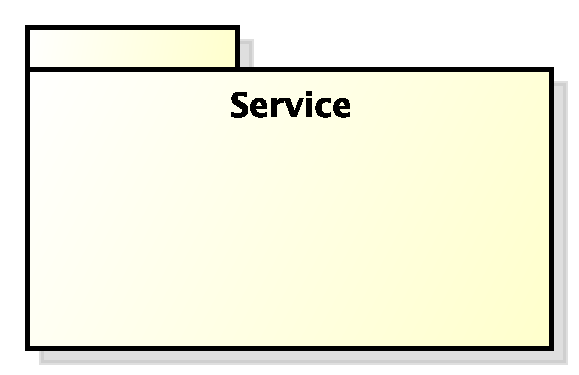
\includegraphics[scale=0.5]{DefinizioneDiProdotto/Pics/Classi/Applicazione--Model--Service}
				\caption{Applicazione::Model::Service}
			\end{figure}
		}
	

			\begin{itemize}
			\item \textbf{Nome:} Service
			\item \textbf{Tipo:} package
			
			\item \textbf{Descrizione:} Il package Service mette a disposizione le funzionalità per l'invio e la ricezione di eventi attraverso canale socket tra l'applicazione e il server.
			\end{itemize}

			
			\level{5}[ChartReceiver]{Applicazione::Model::Service::ChartReceiver}
			

		\IfFileExists{DefinizioneDiProdotto/Pics/Classi/Applicazione--Model--Service--ChartReceiver.pdf}{
			\begin{figure}[H]
				\centering
				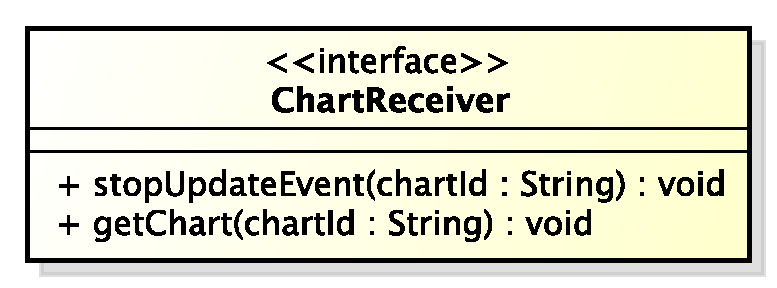
\includegraphics[scale=0.5]{DefinizioneDiProdotto/Pics/Classi/Applicazione--Model--Service--ChartReceiver}
				\caption{Applicazione::Model::Service::ChartReceiver}
			\end{figure}
		}
	
			
			\begin{itemize}
			\item \textbf{Nome:} ChartReceiver
			\item \textbf{Tipo:} interfaccia
			
			\item \textbf{Visibilità:} public
			\item \textbf{Descrizione:} ChartReceiver è l'interfaccia di ChartReceiverImpl.
			\item \textbf{Metodi:}
				\begin{itemize}
				\setlength{\itemsep}{5pt}
				
					\item[\ding{111}] {{+stopUpdateEvent(chartId : String) : void}} \\ [1mm] Tale metodo ha il compito di terminare la ricezione degli aggiornamenti attraverso il canale socket per il chart con id idchart.
					\item[\ding{111}] {{+getChart(chartId : String) : void}} \\ [1mm] Tale metodo ha il compito di reperire dati e impostazioni di un chart il cui id è chartId. Tale metodo ritorna un HashMap nel quale sono salvati tali dati con le chiavi "data" e "settings".
				\end{itemize}
		
			\end{itemize}

			
			\level{5}[ChartReceiverImpl]{Applicazione::Model::Service::ChartReceiverImpl}
			

		\IfFileExists{DefinizioneDiProdotto/Pics/Classi/Applicazione--Model--Service--ChartReceiverImpl.pdf}{
			\begin{figure}[H]
				\centering
				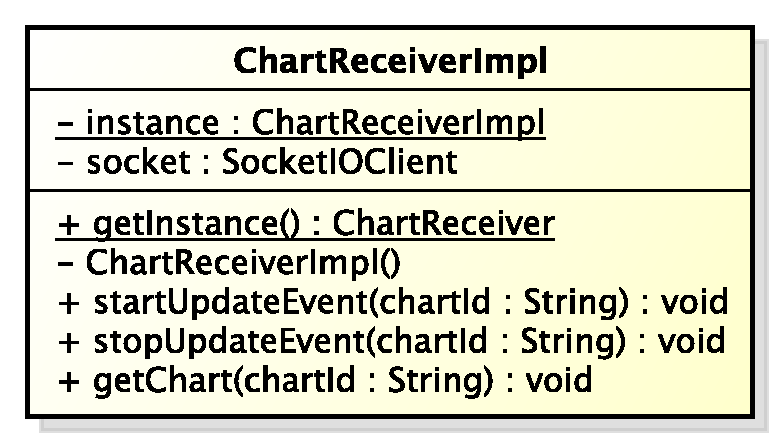
\includegraphics[scale=0.5]{DefinizioneDiProdotto/Pics/Classi/Applicazione--Model--Service--ChartReceiverImpl}
				\caption{Applicazione::Model::Service::ChartReceiverImpl}
			\end{figure}
		}
	
			
			\begin{itemize}
			\item \textbf{Nome:} ChartReceiverImpl
			\item \textbf{Tipo:} classe
			
		\item \textbf{Estende:}
		Observable
		\item \textbf{Implementa:}
		ChartReceiver
		\item \textbf{Astratta:}
		no
			\item \textbf{Visibilità:} public
			\item \textbf{Descrizione:} Tale classe ha il compito di comunicare e ricevere eventi attraverso il canale socket tra app e server. Possono essere avviati o stoppati gli aggiornamenti oppure può esser fatta la richiesta du un intero chart attraverso le api esterne di Norris. Tale classe estende la classe Observable della JDK.
			\item \textbf{Attributi:}
				\begin{itemize}
				\setlength{\itemsep}{5pt}
				
					\item[\ding{111}] \underline{--instance : ChartReceiverImpl} \\ [1mm] Tale attributo statico rappresenta l'istanza univoca di tale classe.
					\item[\ding{111}] {--socket : SocketIOClient} \\ [1mm] Tale attributo rappresenta l'istanza del socket connesso con il server dell'istanza di Norris.
				\end{itemize}
		
			\item \textbf{Metodi:}
				\begin{itemize}
				\setlength{\itemsep}{5pt}
				
					\item[\ding{111}] {\underline{+getInstance() : ChartReceiver}} \\ [1mm] Tale metodo ha il compito di ritornare l'istanza unica di tale classe e se non esiste la crea.
					\item[\ding{111}] {{--ChartReceiverImpl()}} \\ [1mm] Tale metodo è il costruttore della classe. Esso è privato perchè non si vuole permettere a nessuno di poter creare un'istanza se non utilizzando il metodo getInstance().
					\item[\ding{111}] {{+stopUpdateEvent(chartId : String) : void}} \\ [1mm] Tale metodo ha il compito di terminare la ricezione degli aggiornamenti attraverso il canale socket per il chart con id idchart.
					\item[\ding{111}] {{+getChart(chartId : String) : void}} \\ [1mm] Tale metodo ha il compito di reperire dati e impostazioni di un chart il cui id è chartId. Attiva inoltre la ricezione degli aggiornamenti tramite socket event. Imposta dunque una callback che avverta gli osservatori di avvenuta ricezione.
				\end{itemize}
		
			\end{itemize}

			
			\level{4}[View]{Applicazione::View}
			

		\IfFileExists{DefinizioneDiProdotto/Pics/Classi/Applicazione--View.pdf}{
			\begin{figure}[H]
				\centering
				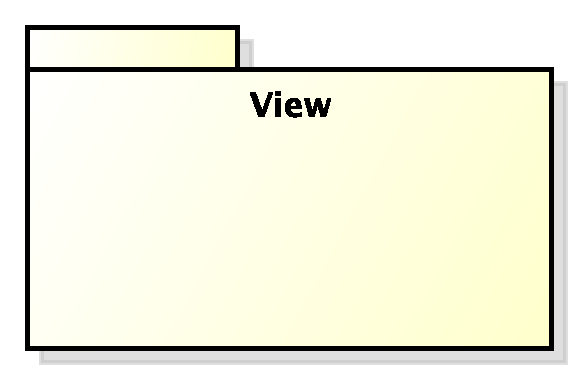
\includegraphics[scale=0.5]{DefinizioneDiProdotto/Pics/Classi/Applicazione--View}
				\caption{Applicazione::View}
			\end{figure}
		}
	

			\begin{itemize}
			\item \textbf{Nome:} View
			\item \textbf{Tipo:} package
			
			\item \textbf{Descrizione:} Le classi del package View rappresentano le UI dell'applicazione, ognuna delle quali mette a disposizione i metodi necessari per modificarla. Ogni user gesture rilevata viene inviata al presenter che si occuperà di gestirla correttamente. 
			\end{itemize}

			
			\level{5}[BarChartActivity]{Applicazione::View::BarChartActivity}
			

		\IfFileExists{DefinizioneDiProdotto/Pics/Classi/Applicazione--View--BarChartActivity.pdf}{
			\begin{figure}[H]
				\centering
				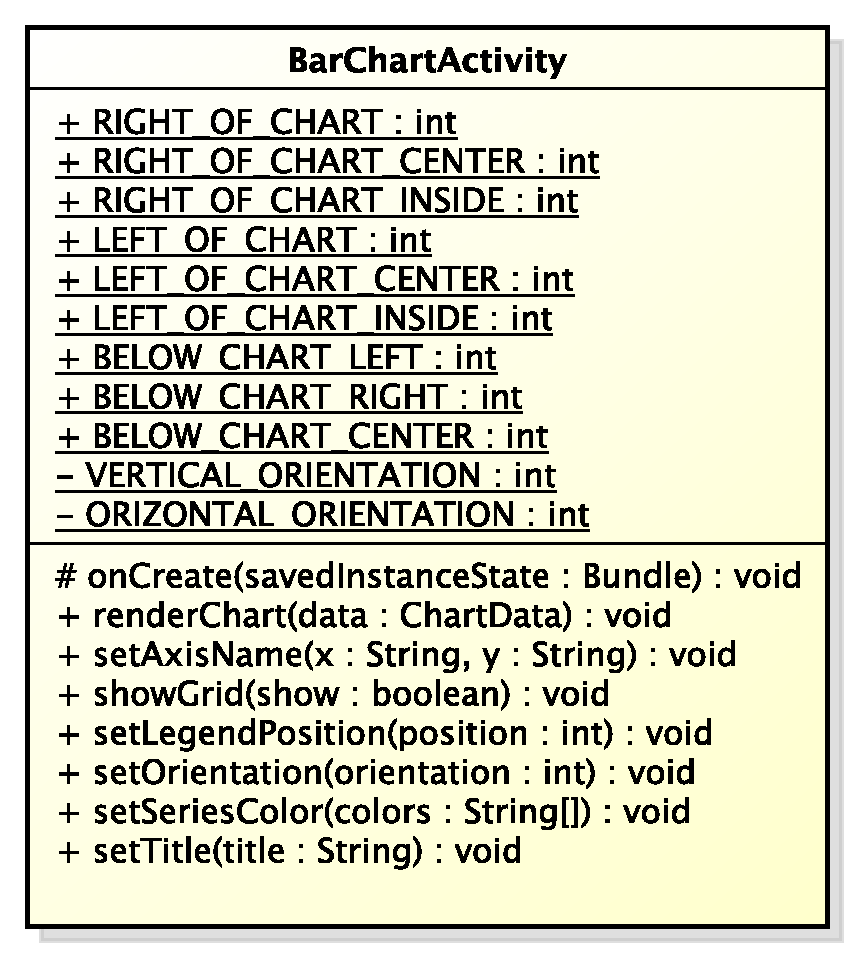
\includegraphics[scale=0.5]{DefinizioneDiProdotto/Pics/Classi/Applicazione--View--BarChartActivity}
				\caption{Applicazione::View::BarChartActivity}
			\end{figure}
		}
	
			
			\begin{itemize}
			\item \textbf{Nome:} BarChartActivity
			\item \textbf{Tipo:} classe
			
		\item \textbf{Estende:}
		ChartActivity
		\item \textbf{Implementa:}
		BarChartView
		\item \textbf{Astratta:}
		no
			\item \textbf{Visibilità:} public
			\item \textbf{Descrizione:} BarChartActivity specializza ChartActivity e costituice un'activity per i grafici di tipo bar chart. Essa mette a disposizione delle costanti statiche che rappresentano i valori possibili da passare ai metodi per modificare la view.
			\item \textbf{Metodi:}
				\begin{itemize}
				\setlength{\itemsep}{5pt}
				
					\item[\ding{111}] {{\#onCreate(savedInstanceState : Bundle) : void}} \\ [1mm] Tale metodo viene eseguito da android alla creazione dell'Activity. Esso avrà il compito di inizializzare il relativo presenter. 
					\item[\ding{111}] {{\#onResume() : void}} \\ [1mm] Tale metodo viene eseguito da android qualora l'activity viene renderizzata. Questo avviene per esempio quando viene ruotato lo schermo passando da landscape a portrait e viceversa o quando l'activity riottiene il foreground. Viene quindi avvertito il presenter di tale evento lasciando a lui la responsabilità sul da farsi.
					\item[\ding{111}] {{\#onPause() : void}} \\ [1mm] Tale metodo viene eseguito da android quando l'activity non possiede piu il foreground. Tale metodo quindi dovrà avvertire il presenter di tale evento e sarà lui a decidere come comportarsi.
					\item[\ding{111}] {{+renderChart(data : ChartData) : void}} \\ [1mm] Tale metodo ha il compito di rappresentare i dati del chart passati come parametro mantenendo quindi aggiornata la visualizzazione all'utente.
					\item[\ding{111}] {{+setAxisName(x : String, y : String) : void}} \\ [1mm] Tale metodo mette a disposizione la possibilità di visualizzare nella view il nome degli assi del chart.
					\item[\ding{111}] {{+showGrid(show : boolean) : void}} \\ [1mm] Tale metodo mette a disposizione la possibilità di visualizzare o no la griglia nel chart. Se il parametro è true viene visualizzata e viene nascosta altrimenti.
					\item[\ding{111}] {{+setLegendPosition(position : int) : void}} \\ [1mm] Tale metodo mette a disposizione la possibilità di imposare la posizione della legenda. Le posizione ammissibili sono 5: a destra, sinistra, sopra, sotto e internamente. Vi è inoltre la possibilità di nascondere la leggenda dando il valore 0.
					\item[\ding{111}] {{+setOrientation(orientation : String) : void}} \\ [1mm] Tale metodo mette a disposizione la possibilità di modificare l'orientamento del chart in base al parametro. I valori passati come parametro possono essere le stringhe "vertical" o "horizontal". In base a tale valore dovrà esser modificata la visualizzazione del chart.
					\item[\ding{111}] {{+setBarValueSpacing(barValueSpacing : int) : void}} \\ [1mm] Tale metodo ha il compito di impostare lo spazio tra due barre del grafico. Il valore dello spazio tra queste dovrà essere impostato a seconda delvalore del parametro passato.
					\item[\ding{111}] {{+setBarDataSetSpacing(barDataSetSpacing : int) : void}} \\ [1mm] Tale metodo ha il compito di impostare lo spazio tra due gruppi di set del grafico. Il valore dello spazio tra i gruppi che dovrà essere impostato viene passato come parametro.
				\end{itemize}
		
			\end{itemize}

			
			\level{5}[BarChartView]{Applicazione::View::BarChartView}
			

		\IfFileExists{DefinizioneDiProdotto/Pics/Classi/Applicazione--View--BarChartView.pdf}{
			\begin{figure}[H]
				\centering
				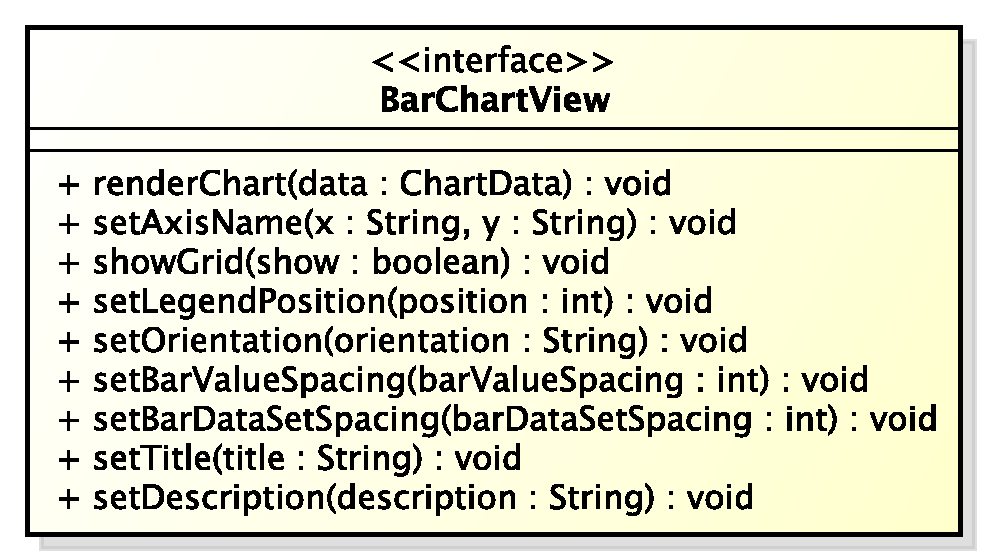
\includegraphics[scale=0.5]{DefinizioneDiProdotto/Pics/Classi/Applicazione--View--BarChartView}
				\caption{Applicazione::View::BarChartView}
			\end{figure}
		}
	
			
			\begin{itemize}
			\item \textbf{Nome:} BarChartView
			\item \textbf{Tipo:} interfaccia
			
		\item \textbf{Estende:}
		View
			\item \textbf{Visibilità:} public
			\item \textbf{Descrizione:} Tale interfaccia ha il compito di permettere l'utilizzo dei metodi per modificare la view per rappresentare un bar chart dall'esterno del package View (quindi da un BarChartPresenterImpl).
			\item \textbf{Metodi:}
				\begin{itemize}
				\setlength{\itemsep}{5pt}
				
					\item[\ding{111}] {{+renderChart(data : ChartData) : void}} \\ [1mm] Tale metodo ha il compito di rappresentare i dati del chart passati come parametro mantenendo quindi aggiornata la visualizzazione all'utente.
					\item[\ding{111}] {{+setAxisName(x : String, y : String) : void}} \\ [1mm] Tale metodo mette a disposizione la possibilità di visualizzare nella view il nome degli assi del chart.
					\item[\ding{111}] {{+showGrid(show : boolean) : void}} \\ [1mm] Tale metodo mette a disposizione la possibilità di visualizzare o no la griglia nel chart. Se il parametro è true viene visualizzata e viene nascosta altrimenti.
					\item[\ding{111}] {{+setLegendPosition(position : int) : void}} \\ [1mm] Tale metodo mette a disposizione la possibilità di imposare la posizione della legenda. Le posizione ammissibili sono 5: a destra, sinistra, sopra, sotto e internamente. Vi è inoltre la possibilità di nascondere la leggenda dando il valore 0.
					\item[\ding{111}] {{+setOrientation(orientation : String) : void}} \\ [1mm] Tale metodo mette a disposizione la possibilità di modificare l'orientamento del chart in base al parametro. I valori passati come parametro possono essere le stringhe "vertical" o "horizontal". In base a tale valore dovrà esser modificata la visualizzazione del chart.
					\item[\ding{111}] {{+setBarValueSpacing(barValueSpacing : int) : void}} \\ [1mm] Tale metodo ha il compito di impostare lo spazio tra due barre del grafico. Il valore dello spazio tra queste dovrà essere impostato a seconda delvalore del parametro passato.
					\item[\ding{111}] {{+setBarDataSetSpacing(barDataSetSpacing : int) : void}} \\ [1mm] Tale metodo ha il compito di impostare lo spazio tra due gruppi di set del grafico. Il valore dello spazio tra i gruppi che dovrà essere impostato viene passato come parametro.
					\item[\ding{111}] {{+setTitle(title : String) : void}} \\ [1mm] Tale metodo ha il compito di visualizzare il titolo del chart. Dovrà quindi esser visualizzato sulla action bar il titolo ricevuto come parametro.
					\item[\ding{111}] {{+setDescription(description : String) : void}} \\ [1mm] Tale metodo ha il compito di visualizzare il titolo del chart. Dovrà quindi esser visualizzato come sottotitolo della action bar la descrizione ricevuta come parametro.
				\end{itemize}
		
			\end{itemize}

			
			\level{5}[BaseActivity]{Applicazione::View::BaseActivity}
			

		\IfFileExists{DefinizioneDiProdotto/Pics/Classi/Applicazione--View--BaseActivity.pdf}{
			\begin{figure}[H]
				\centering
				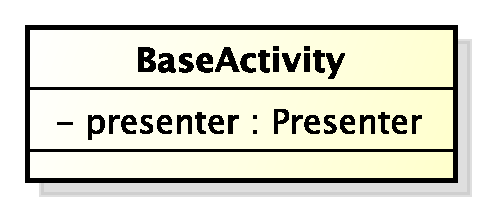
\includegraphics[scale=0.5]{DefinizioneDiProdotto/Pics/Classi/Applicazione--View--BaseActivity}
				\caption{Applicazione::View::BaseActivity}
			\end{figure}
		}
	
			
			\begin{itemize}
			\item \textbf{Nome:} BaseActivity
			\item \textbf{Tipo:} classe
			
		\item \textbf{Estende:}
		ActionBarActivity
		\item \textbf{Astratta:}
		si
			\item \textbf{Visibilità:} public
			\item \textbf{Descrizione:} Tale classe rappresenta l'astrazione di un'activity. Essa contiene il riferimento al presenter generico che sarà instanziato dalle specializzazioni di tale classe.
			\item \textbf{Attributi:}
				\begin{itemize}
				\setlength{\itemsep}{5pt}
				
					\item[\ding{111}] {\#presenter : Presenter}
				\end{itemize}
		
			\end{itemize}

			
			\level{5}[ChartActivity]{Applicazione::View::ChartActivity}
			

		\IfFileExists{DefinizioneDiProdotto/Pics/Classi/Applicazione--View--ChartActivity.pdf}{
			\begin{figure}[H]
				\centering
				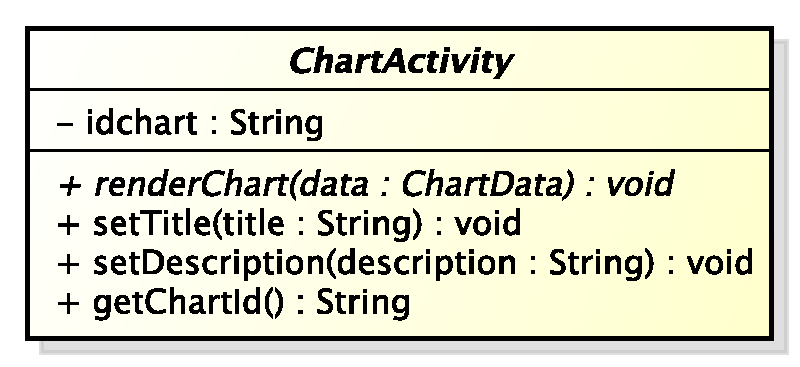
\includegraphics[scale=0.5]{DefinizioneDiProdotto/Pics/Classi/Applicazione--View--ChartActivity}
				\caption{Applicazione::View::ChartActivity}
			\end{figure}
		}
	
			
			\begin{itemize}
			\item \textbf{Nome:} ChartActivity
			\item \textbf{Tipo:} classe
			
		\item \textbf{Estende:}
		BaseActivity
		\item \textbf{Astratta:}
		si
			\item \textbf{Visibilità:} package
			\item \textbf{Descrizione:} ChartActivity è una classe astratta che rappresenta un'activity per la rappresentazione di chart generica.
			\item \textbf{Attributi:}
				\begin{itemize}
				\setlength{\itemsep}{5pt}
				
					\item[\ding{111}] {--idchart : String}
				\end{itemize}
		
			\item \textbf{Metodi:}
				\begin{itemize}
				\setlength{\itemsep}{5pt}
				
					\item[\ding{111}] \textit{{+renderChart(data : ChartData) : void}} \\ [1mm] Tale metodo è astratto e tutte le specializzazioni di tale classe devono implementarlo. Esso dovrà visualizzare nel modo corretto il chart.
					\item[\ding{111}] {{+setTitle(title : String) : void}} \\ [1mm] Tale metodo ha il compito di visualizzare il titolo del chart. Dovrà quindi esser visualizzato sulla action bar il titolo ricevuto come parametro.
					\item[\ding{111}] {{+setDescription(description : String) : void}} \\ [1mm] Tale metodo ha il compito di visualizzare il titolo del chart. Dovrà quindi esser visualizzato come sottotitolo della action bar la descrizione ricevuta come parametro.
					\item[\ding{111}] {{+getChartId() : String}} \\ [1mm] Tale metodo ritorna l'id del grafico rappresentato.
				\end{itemize}
		
			\end{itemize}

			
			\level{5}[LineChartActivity]{Applicazione::View::LineChartActivity}
			

		\IfFileExists{DefinizioneDiProdotto/Pics/Classi/Applicazione--View--LineChartActivity.pdf}{
			\begin{figure}[H]
				\centering
				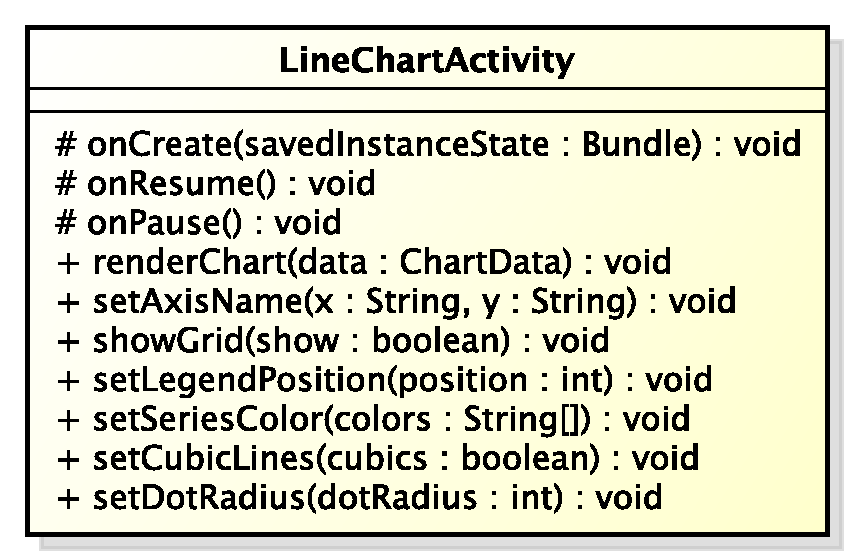
\includegraphics[scale=0.5]{DefinizioneDiProdotto/Pics/Classi/Applicazione--View--LineChartActivity}
				\caption{Applicazione::View::LineChartActivity}
			\end{figure}
		}
	
			
			\begin{itemize}
			\item \textbf{Nome:} LineChartActivity
			\item \textbf{Tipo:} classe
			
		\item \textbf{Estende:}
		ChartActivity
		\item \textbf{Implementa:}
		LineChartView
		\item \textbf{Astratta:}
		no
			\item \textbf{Visibilità:} public
			\item \textbf{Descrizione:} LineChartActivity specializza ChartActivity e costituisce un'activity per i grafici di tipo line chart. Essa mette a disposizione delle costanti statiche che rappresentano i valori possibili da passare ai metodi per modificare la view.
			\item \textbf{Metodi:}
				\begin{itemize}
				\setlength{\itemsep}{5pt}
				
					\item[\ding{111}] {{\#onCreate(savedInstanceState : Bundle) : void}} \\ [1mm] Tale metodo viene eseguito da android alla creazione dell'Activity. Esso avrà il compito di inizializzare il relativo presenter. 
					\item[\ding{111}] {{\#onResume() : void}} \\ [1mm] Tale metodo viene eseguito da android qualora l'activity viene renderizzata. Questo avviene per esempio quando viene ruotato lo schermo passando da landscape a portrait e viceversa o quando l'activity riottiene il foreground. Viene quindi avvertito il presenter di tale evento lasciando a lui la responsabilità sul da farsi.
					\item[\ding{111}] {{\#onPause() : void}} \\ [1mm] Tale metodo viene eseguito da android quando l'activity non possiede piu il foreground. Tale metodo quindi dovrà avvertire il presenter di tale evento e sarà lui a decidere come comportarsi.
					\item[\ding{111}] {{+renderChart(data : ChartData) : void}} \\ [1mm] Tale metodo ha il compito di rappresentare i dati del chart passati come parametro mantenendo quindi aggiornata la visualizzazione all'utente.
					\item[\ding{111}] {{+setAxisName(x : String, y : String) : void}} \\ [1mm] Tale metodo mette a disposizione la possibilità di visualizzare nella view il nome degli assi del chart. Il parametro x rappresenta cosa dovrà esser scritto sull'ettichetta dell'asse delle ascisse mentre il parametro y ciò che andrà su quella delle ascisse.
					\item[\ding{111}] {{+showGrid(show : boolean) : void}} \\ [1mm] Tale metodo mette a disposizione la possibilità di visualizzare o no la griglia nel chart. Se il parametro è true viene visualizzata e viene nascosta altrimenti.
					\item[\ding{111}] {{+setLegendPosition(position : int) : void}} \\ [1mm] Tale metodo mette a disposizione la possibilità di imposare la posizione della legenda. Le posizione ammissibili sono 5: a destra, sinistra, sopra, sotto e internamente. Vi è inoltre la possibilità di nascondere la leggenda dando il valore 0.
					\item[\ding{111}] {{+setCubicLines(cubics : boolean) : void}} \\ [1mm] Tale metodo permette di visualizzare le linee del line chart cubiche o no (a seconda del parametro booleano). Eseguendo tale metodo quindi verrà modificata la visualizzazione del linechart.
					\item[\ding{111}] {{+setDotRadius(dotRadius : int) : void}} \\ [1mm] Tale metodo permette di impostare la dimensione dei punti dei dati. Impostando questo valore a 0 non verranno quindi visualizzati.
				\end{itemize}
		
			\end{itemize}

			
			\level{5}[LineChartView]{Applicazione::View::LineChartView}
			

		\IfFileExists{DefinizioneDiProdotto/Pics/Classi/Applicazione--View--LineChartView.pdf}{
			\begin{figure}[H]
				\centering
				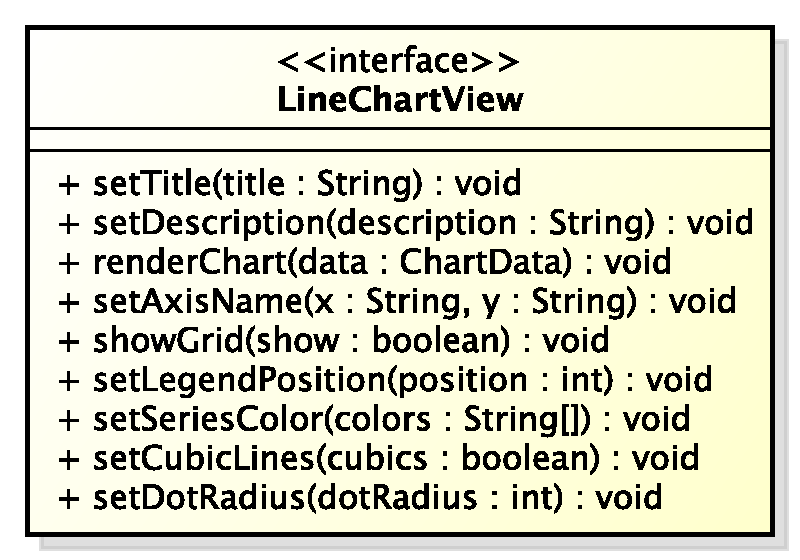
\includegraphics[scale=0.5]{DefinizioneDiProdotto/Pics/Classi/Applicazione--View--LineChartView}
				\caption{Applicazione::View::LineChartView}
			\end{figure}
		}
	
			
			\begin{itemize}
			\item \textbf{Nome:} LineChartView
			\item \textbf{Tipo:} interfaccia
			
		\item \textbf{Estende:}
		View
			\item \textbf{Visibilità:} public
			\item \textbf{Descrizione:} Tale interfaccia ha il compito di permettere l'utilizzo dei metodi per modificare la view per rappresentare un line chart dall'esterno del package View (quindi da un LineChartPresenterImpl).
			\item \textbf{Metodi:}
				\begin{itemize}
				\setlength{\itemsep}{5pt}
				
					\item[\ding{111}] {{+renderChart(data : ChartData) : void}} \\ [1mm] Tale metodo ha il compito di rappresentare i dati del chart passati come parametro mantenendo quindi aggiornata la visualizzazione all'utente.
					\item[\ding{111}] {{+setAxisName(x : String, y : String) : void}} \\ [1mm] Tale metodo mette a disposizione la possibilità di visualizzare nella view il nome degli assi del chart. Il parametro x rappresenta cosa dovrà esser scritto sull'ettichetta dell'asse delle ascisse mentre il parametro y ciò che andrà su quella delle ascisse.
					\item[\ding{111}] {{+showGrid(show : boolean) : void}} \\ [1mm] Tale metodo mette a disposizione la possibilità di visualizzare o no la griglia nel chart. Se il parametro è true viene visualizzata e viene nascosta altrimenti.
					\item[\ding{111}] {{+setLegendPosition(position : int) : void}} \\ [1mm] Tale metodo mette a disposizione la possibilità di imposare la posizione della legenda. Le posizione ammissibili sono 5: a destra, sinistra, sopra, sotto e internamente. Vi è inoltre la possibilità di nascondere la leggenda dando il valore 0.
					\item[\ding{111}] {{+setCubicLines(cubics : boolean) : void}} \\ [1mm] Tale metodo permette di visualizzare le linee del line chart cubiche o no (a seconda del parametro booleano). Eseguendo tale metodo quindi verrà modificata la visualizzazione del linechart.
					\item[\ding{111}] {{+setDotRadius(dotRadius : int) : void}} \\ [1mm] Tale metodo permette di impostare la dimensione dei punti dei dati. Impostando questo valore a 0 non verranno quindi visualizzati.
					\item[\ding{111}] {{+setTitle(title : String) : void}} \\ [1mm] Tale metodo ha il compito di visualizzare il titolo del chart. Dovrà quindi esser visualizzato sulla action bar il titolo ricevuto come parametro.
					\item[\ding{111}] {{+setDescription(description : String) : void}} \\ [1mm] Tale metodo ha il compito di visualizzare il titolo del chart. Dovrà quindi esser visualizzato come sottotitolo della action bar la descrizione ricevuta come parametro.
				\end{itemize}
		
			\end{itemize}

			
			\level{5}[ListActivity]{Applicazione::View::ListActivity}
			

		\IfFileExists{DefinizioneDiProdotto/Pics/Classi/Applicazione--View--ListActivity.pdf}{
			\begin{figure}[H]
				\centering
				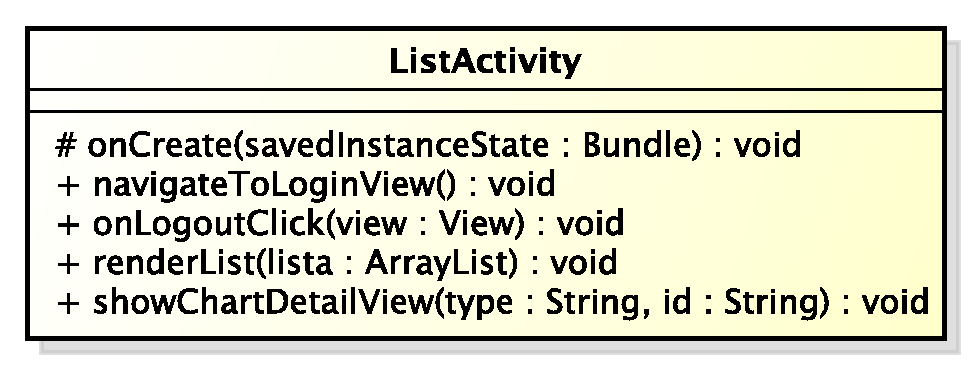
\includegraphics[scale=0.5]{DefinizioneDiProdotto/Pics/Classi/Applicazione--View--ListActivity}
				\caption{Applicazione::View::ListActivity}
			\end{figure}
		}
	
			
			\begin{itemize}
			\item \textbf{Nome:} ListActivity
			\item \textbf{Tipo:} classe
			
		\item \textbf{Estende:}
		BaseActivity
		\item \textbf{Implementa:}
		ListView
		\item \textbf{Astratta:}
		no
			\item \textbf{Visibilità:} public
			\item \textbf{Descrizione:} ListActivity si occupa di mostrare la lista dei grafici contenuti in un'istanza di Norris. Ogni elemento della lista rappresenterà un chart dell'istanza che cliccato e avvertirà il relativo presenter della user gesture.
			\item \textbf{Metodi:}
				\begin{itemize}
				\setlength{\itemsep}{5pt}
				
					\item[\ding{111}] {{\#onCreate(savedInstanceState : Bundle) : void}} \\ [1mm] Tale metodo viene eseguito da android alla creazione dell'Activity. Esso avrà il compito di inizializzare il relativo presenter. 
					\item[\ding{111}] {{+navigateToLoginView() : void}} \\ [1mm] Tale metodo avvia l'activity home. Essa viene richiamata dal presenter qualora l'utente effettua il logout.
					\item[\ding{111}] {{+onLogoutClick(view : View) : void}} \\ [1mm] Tale metodo viene invocato in automatico da Android qualora viene cliccato il bottone di logout. Esso avvertirà il relativo presenter dell'avvenuta pressione.
					\item[\ding{111}] {{+renderList(lista : ArrayList) : void}} \\ [1mm] Tale metodo viene invocato con lo scopo di popolare la list view. I dati con i quali deve esser popolata sono presenti nell'ArrayList passato come parametro. Ogni elemento di tale array con
					\item[\ding{111}] {{+showChartDetailView(type : String, id : String) : void}} \\ [1mm] Tale metodo avvia l'activity nella quale sarà presente il dettaglio di un chart specifico. La scelta di quale activity avviare spetta ad esso.
				\end{itemize}
		
			\end{itemize}

			
			\level{5}[ListView]{Applicazione::View::ListView}
			

		\IfFileExists{DefinizioneDiProdotto/Pics/Classi/Applicazione--View--ListView.pdf}{
			\begin{figure}[H]
				\centering
				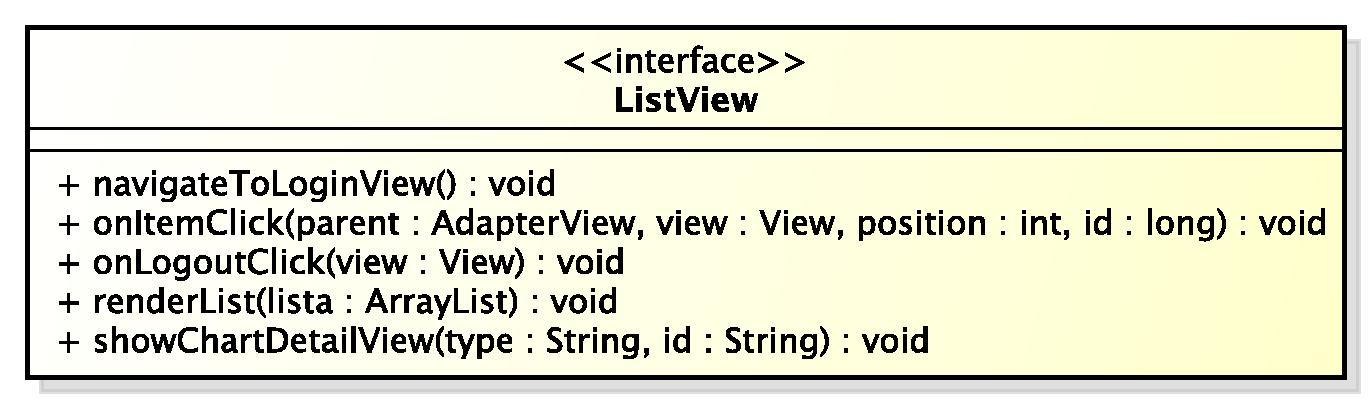
\includegraphics[scale=0.5]{DefinizioneDiProdotto/Pics/Classi/Applicazione--View--ListView}
				\caption{Applicazione::View::ListView}
			\end{figure}
		}
	
			
			\begin{itemize}
			\item \textbf{Nome:} ListView
			\item \textbf{Tipo:} interfaccia
			
		\item \textbf{Estende:}
		View
			\item \textbf{Visibilità:} public
			\item \textbf{Descrizione:} Tale interfaccia ha il compito di permettere l'utilizzo dei metodi per modificare la view con la lista dei chart dall'esterno del package View (quindi da un ListPresenterImpl).
			\end{itemize}

			
			\level{5}[LoginActivity]{Applicazione::View::LoginActivity}
			

		\IfFileExists{DefinizioneDiProdotto/Pics/Classi/Applicazione--View--LoginActivity.pdf}{
			\begin{figure}[H]
				\centering
				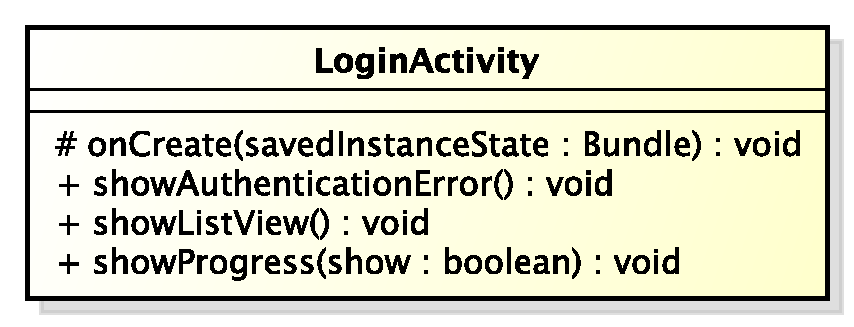
\includegraphics[scale=0.5]{DefinizioneDiProdotto/Pics/Classi/Applicazione--View--LoginActivity}
				\caption{Applicazione::View::LoginActivity}
			\end{figure}
		}
	
			
			\begin{itemize}
			\item \textbf{Nome:} LoginActivity
			\item \textbf{Tipo:} classe
			
		\item \textbf{Estende:}
		BaseActivity
		\item \textbf{Implementa:}
		LoginView
		\item \textbf{Astratta:}
		no
			\item \textbf{Visibilità:} public
			\item \textbf{Descrizione:} LoginActivity si occupa di mostrare la schermata di autenticazione, in cui l'utente può inserire l'indirizzo dell'istanza di Norris, username e password. Qualora l'utente clicchi il tasto di login verrà avvertito il relativo presenter che si occuperà della richiesta.
			\item \textbf{Metodi:}
				\begin{itemize}
				\setlength{\itemsep}{5pt}
				
					\item[\ding{111}] {{\#onCreate(savedInstanceState : Bundle) : void}} \\ [1mm] Tale metodo viene eseguito da android alla creazione dell'Activity. Esso avrà il compito di inizializzare il relativo presenter. 
					\item[\ding{111}] {{+showAuthenticationError(err : String) : void}} \\ [1mm] Tale metodo mostra nella view l'avvenuto errore stampando la stringa passata come parametro.
					\item[\ding{111}] {{+showListView() : void}} \\ [1mm] Tale metodo avvia l'activity nella quale sarà presente la lista con i chart dell'istaza di Norris.
					\item[\ding{111}] {{+showProgress(show : boolean) : void}} \\ [1mm] Tale metodo visualizza sulla view un segnale di attesa se il parametro è true e lo nasconde altrimenti.
					\item[\ding{111}] {{+onLoginClick(view : View) : void}} \\ [1mm] Tale metodo viene invocato in automatico da android qualora viene cliccato il bottone di login. Esso avvertirà il relativo presenter dell'avvenuta pressione.
				\end{itemize}
		
			\end{itemize}

			
			\level{5}[LoginView]{Applicazione::View::LoginView}
			

		\IfFileExists{DefinizioneDiProdotto/Pics/Classi/Applicazione--View--LoginView.pdf}{
			\begin{figure}[H]
				\centering
				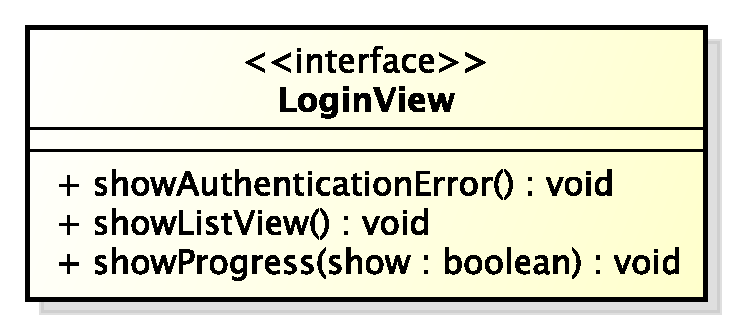
\includegraphics[scale=0.5]{DefinizioneDiProdotto/Pics/Classi/Applicazione--View--LoginView}
				\caption{Applicazione::View::LoginView}
			\end{figure}
		}
	
			
			\begin{itemize}
			\item \textbf{Nome:} LoginView
			\item \textbf{Tipo:} interfaccia
			
		\item \textbf{Estende:}
		View
			\item \textbf{Visibilità:} public
			\item \textbf{Descrizione:} Tale interfaccia ha il compito di permettere l'utilizzo dei metodi per modificare la view di login dall'esterno del package View (quindi da un LoginPresenterImpl).
			\end{itemize}

			
			\level{5}[MapChartActivity]{Applicazione::View::MapChartActivity}
			

		\IfFileExists{DefinizioneDiProdotto/Pics/Classi/Applicazione--View--MapChartActivity.pdf}{
			\begin{figure}[H]
				\centering
				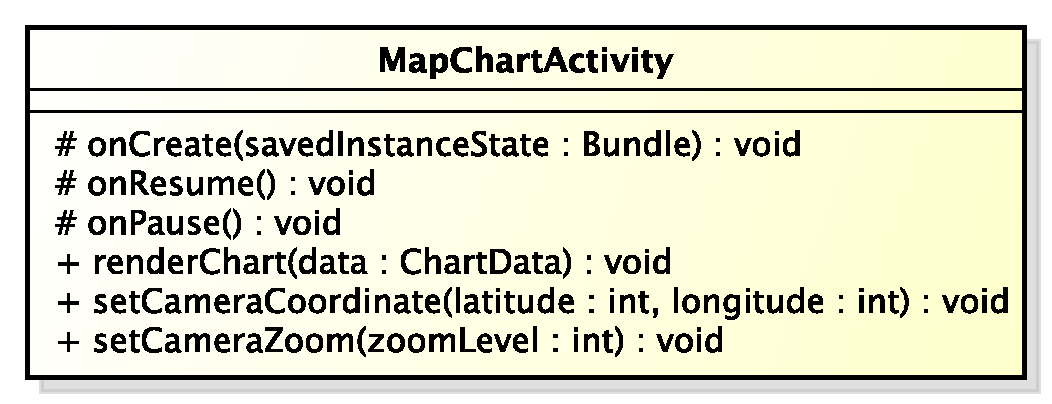
\includegraphics[scale=0.5]{DefinizioneDiProdotto/Pics/Classi/Applicazione--View--MapChartActivity}
				\caption{Applicazione::View::MapChartActivity}
			\end{figure}
		}
	
			
			\begin{itemize}
			\item \textbf{Nome:} MapChartActivity
			\item \textbf{Tipo:} classe
			
		\item \textbf{Estende:}
		ChartActivity
		\item \textbf{Implementa:}
		MapChartView
		\item \textbf{Astratta:}
		no
			\item \textbf{Visibilità:} public
			\item \textbf{Descrizione:} MapChartActivity specializza ChartActivity e costituice un'activity per i grafici di tipo map chart. Essa mette a disposizione delle costanti statiche che rappresentano i valori possibili da passare ai metodi per modificare la view.
			\item \textbf{Metodi:}
				\begin{itemize}
				\setlength{\itemsep}{5pt}
				
					\item[\ding{111}] {{\#onCreate(savedInstanceState : Bundle) : void}} \\ [1mm] Tale metodo viene eseguito da android alla creazione dell'Activity. Esso avrà il compito di inizializzare il relativo presenter. 
					\item[\ding{111}] {{\#onResume() : void}} \\ [1mm] Tale metodo viene eseguito da android qualora l'activity viene renderizzata. Questo avviene per esempio quando viene ruotato lo schermo passando da landscape a portrait e viceversa o quando l'activity riottiene il foreground. Viene quindi avvertito il presenter di tale evento lasciando a lui la responsabilità sul da farsi.
					\item[\ding{111}] {{\#onPause() : void}} \\ [1mm] Tale metodo viene eseguito da android quando l'activity non possiede piu il foreground. Tale metodo quindi dovrà avvertire il presenter di tale evento e sarà lui a decidere come comportarsi.
					\item[\ding{111}] {{+renderChart(data : ChartData) : void}} \\ [1mm] Tale metodo ha il compito di rappresentare i dati del chart passati come parametro mantenendo quindi aggiornata la visualizzazione all'utente.
					\item[\ding{111}] {{+setCameraCoordinate(latitude : int, longitude : int) : void}} \\ [1mm] Tale metodo mette a disposizione la possibilità di modificare la posizione di visualizzazione del map chart, ovvero le coordinate del punto centrale.
					\item[\ding{111}] {{+setCameraZoom(zoomLevel : int) : void}} \\ [1mm] Tale metodo mette a disposizione la possibilità di modificare l'altezza di visualizzazione del map chart. L'altezza da impostare sarà passata come parametro ed essa assumerà valori compresi tra 0 e 19.
				\end{itemize}
		
			\end{itemize}

			
			\level{5}[MapChartView]{Applicazione::View::MapChartView}
			

		\IfFileExists{DefinizioneDiProdotto/Pics/Classi/Applicazione--View--MapChartView.pdf}{
			\begin{figure}[H]
				\centering
				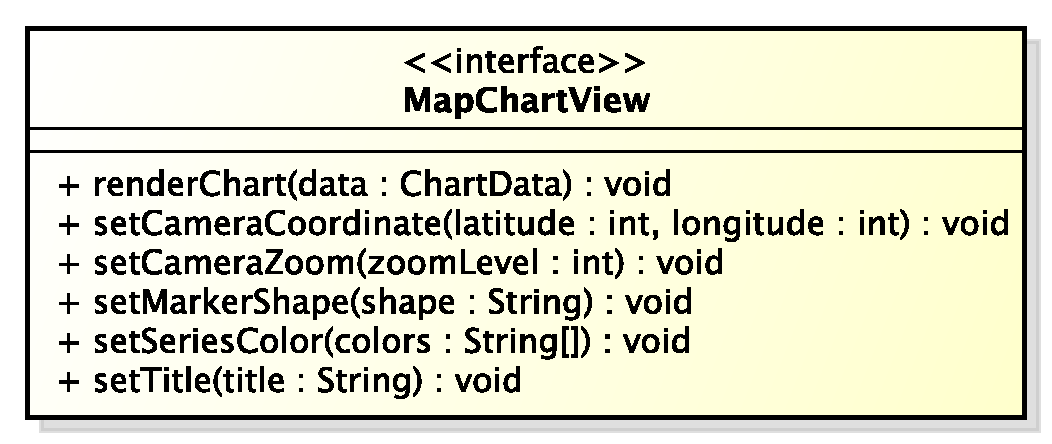
\includegraphics[scale=0.5]{DefinizioneDiProdotto/Pics/Classi/Applicazione--View--MapChartView}
				\caption{Applicazione::View::MapChartView}
			\end{figure}
		}
	
			
			\begin{itemize}
			\item \textbf{Nome:} MapChartView
			\item \textbf{Tipo:} interfaccia
			
		\item \textbf{Estende:}
		View
			\item \textbf{Visibilità:} public
			\item \textbf{Descrizione:} Tale interfaccia ha il compito di permettere l'utilizzo dei metodi per modificare la view per rappresentare un map chart dall'esterno del package View (quindi da un MapChartPresenterImpl).
			\item \textbf{Metodi:}
				\begin{itemize}
				\setlength{\itemsep}{5pt}
				
					\item[\ding{111}] {{+renderChart(data : ChartData) : void}} \\ [1mm] Tale metodo ha il compito di rappresentare i dati del chart passati come parametro mantenendo quindi aggiornata la visualizzazione all'utente.
					\item[\ding{111}] {{+setCameraCoordinate(latitude : int, longitude : int) : void}} \\ [1mm] Tale metodo mette a disposizione la possibilità di modificare la posizione di visualizzazione del map chart, ovvero le coordinate del punto centrale.
					\item[\ding{111}] {{+setCameraZoom(zoomLevel : int) : void}} \\ [1mm] Tale metodo mette a disposizione la possibilità di modificare l'altezza di visualizzazione del map chart. L'altezza da impostare sarà passata come parametro ed essa assumerà valori compresi tra 0 e 19.
					\item[\ding{111}] {{+setTitle(title : String) : void}} \\ [1mm] Tale metodo ha il compito di visualizzare il titolo del chart. Dovrà quindi esser visualizzato sulla action bar il titolo ricevuto come parametro.
					\item[\ding{111}] {{+setDescription(description : String) : void}} \\ [1mm] Tale metodo ha il compito di visualizzare il titolo del chart. Dovrà quindi esser visualizzato come sottotitolo della action bar la descrizione ricevuta come parametro.
				\end{itemize}
		
			\end{itemize}

			
			\level{5}[TableActivity]{Applicazione::View::TableActivity}
			

		\IfFileExists{DefinizioneDiProdotto/Pics/Classi/Applicazione--View--TableActivity.pdf}{
			\begin{figure}[H]
				\centering
				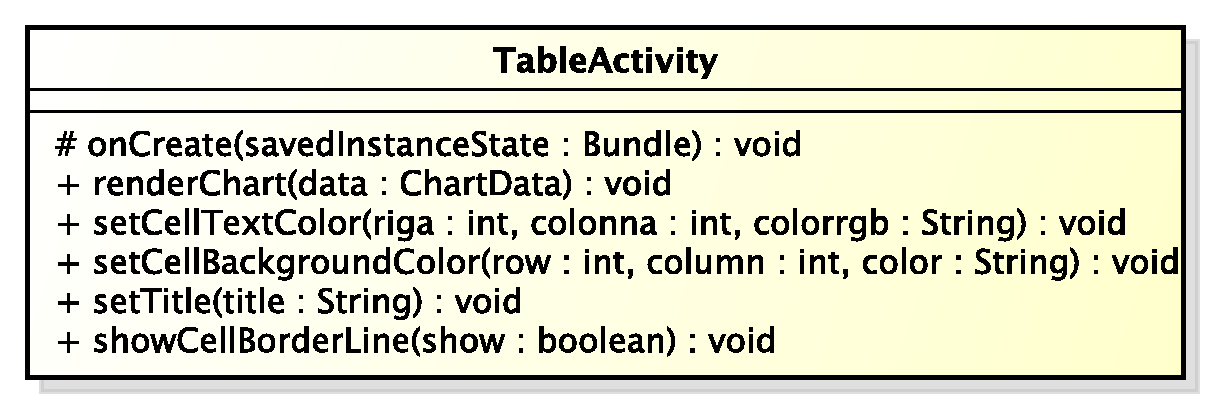
\includegraphics[scale=0.5]{DefinizioneDiProdotto/Pics/Classi/Applicazione--View--TableActivity}
				\caption{Applicazione::View::TableActivity}
			\end{figure}
		}
	
			
			\begin{itemize}
			\item \textbf{Nome:} TableActivity
			\item \textbf{Tipo:} classe
			
		\item \textbf{Estende:}
		ChartActivity
		\item \textbf{Implementa:}
		TableView
		\item \textbf{Astratta:}
		no
			\item \textbf{Visibilità:} public
			\item \textbf{Descrizione:} TableActivity specializza ChartActivity e costituice un'activity per i grafici di tipo table. Essa mette a disposizione delle costanti statiche che rappresentano i valori possibili da passare ai metodi per modificare la view.
			\item \textbf{Metodi:}
				\begin{itemize}
				\setlength{\itemsep}{5pt}
				
					\item[\ding{111}] {{\#onCreate(savedInstanceState : Bundle) : void}} \\ [1mm] Tale metodo viene eseguito da android alla creazione dell'Activity. Esso avrà il compito di inizializzare il relativo presenter. 
					\item[\ding{111}] {{\#onResume() : void}} \\ [1mm] Tale metodo viene eseguito da android qualora l'activity viene renderizzata. Questo avviene per esempio quando viene ruotato lo schermo passando da landscape a portrait e viceversa o quando l'activity riottiene il foreground. Viene quindi avvertito il presenter di tale evento lasciando a lui la responsabilità sul da farsi.
					\item[\ding{111}] {{\#onPause() : void}} \\ [1mm] Tale metodo viene eseguito da android quando l'activity non possiede piu il foreground. Tale metodo quindi dovrà avvertire il presenter di tale evento e sarà lui a decidere come comportarsi.
					\item[\ding{111}] {{+renderChart(data : ChartData) : void}} \\ [1mm] Tale metodo ha il compito di rappresentare i dati del chart passati come parametro mantenendo quindi aggiornata la visualizzazione all'utente.
					\item[\ding{111}] {{+showCellBorderLine(show : boolean) : void}} \\ [1mm] Tale metodo mette a disposizione la possibilità di visualizzare o no le linee dei bordi delle celle della table.
				\end{itemize}
		
			\end{itemize}

			
			\level{5}[TableView]{Applicazione::View::TableView}
			

		\IfFileExists{DefinizioneDiProdotto/Pics/Classi/Applicazione--View--TableView.pdf}{
			\begin{figure}[H]
				\centering
				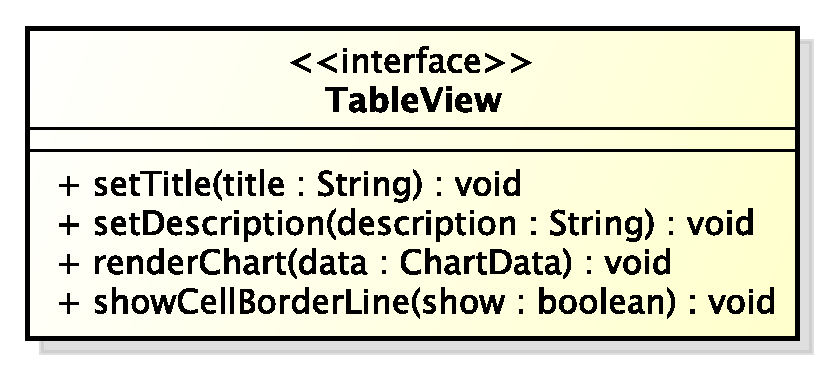
\includegraphics[scale=0.5]{DefinizioneDiProdotto/Pics/Classi/Applicazione--View--TableView}
				\caption{Applicazione::View::TableView}
			\end{figure}
		}
	
			
			\begin{itemize}
			\item \textbf{Nome:} TableView
			\item \textbf{Tipo:} interfaccia
			
		\item \textbf{Estende:}
		View
			\item \textbf{Visibilità:} public
			\item \textbf{Descrizione:} Tale interfaccia ha il compito di permettere l'utilizzo dei metodi per modificare la view per rappresentare una table dall'esterno del package View (quindi da un TablePresenterImpl).
			\item \textbf{Metodi:}
				\begin{itemize}
				\setlength{\itemsep}{5pt}
				
					\item[\ding{111}] {{+renderChart(data : ChartData) : void}} \\ [1mm] Tale metodo ha il compito di rappresentare i dati del chart passati come parametro mantenendo quindi aggiornata la visualizzazione all'utente.
					\item[\ding{111}] {{+showCellBorderLine(show : boolean) : void}} \\ [1mm] Tale metodo mette a disposizione la possibilità di visualizzare o no le linee dei bordi delle celle della table.
					\item[\ding{111}] {{+setTitle(title : String) : void}} \\ [1mm] Tale metodo ha il compito di visualizzare il titolo del chart. Dovrà quindi esser visualizzato sulla action bar il titolo ricevuto come parametro.
					\item[\ding{111}] {{+setDescription(description : String) : void}} \\ [1mm] Tale metodo ha il compito di visualizzare il titolo del chart. Dovrà quindi esser visualizzato come sottotitolo della action bar la descrizione ricevuta come parametro.
				\end{itemize}
		
			\end{itemize}

			
			\level{5}[View]{Applicazione::View::View}
			

		\IfFileExists{DefinizioneDiProdotto/Pics/Classi/Applicazione--View--View.pdf}{
			\begin{figure}[H]
				\centering
				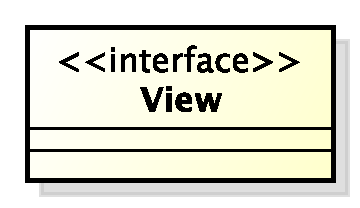
\includegraphics[scale=0.5]{DefinizioneDiProdotto/Pics/Classi/Applicazione--View--View}
				\caption{Applicazione::View::View}
			\end{figure}
		}
	
			
			\begin{itemize}
			\item \textbf{Nome:} View
			\item \textbf{Tipo:} interfaccia
			
			\item \textbf{Visibilità:} public
			\item \textbf{Descrizione:} Tale interfaccia ha il compito di permettere l'utilizzo dei metodi per modificare le varie view dall'esterno del package View (quindi da un particolare presenter).
			\end{itemize}

			
			\level{4}[Presenter]{Applicazione::Presenter}
			

		\IfFileExists{DefinizioneDiProdotto/Pics/Classi/Applicazione--Presenter.pdf}{
			\begin{figure}[H]
				\centering
				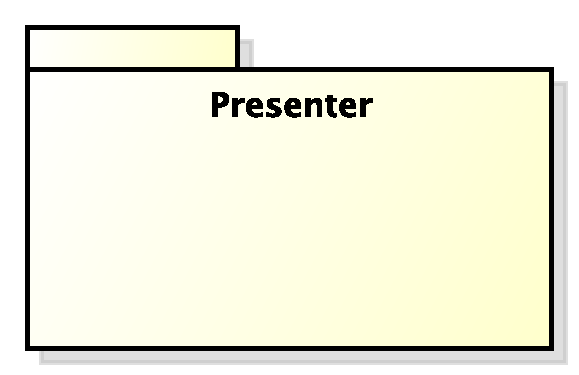
\includegraphics[scale=0.5]{DefinizioneDiProdotto/Pics/Classi/Applicazione--Presenter}
				\caption{Applicazione::Presenter}
			\end{figure}
		}
	

			\begin{itemize}
			\item \textbf{Nome:} Presenter
			\item \textbf{Tipo:} package
			
			\item \textbf{Descrizione:} Il package Presenter contiene le classi che hanno il compito di gestire l'intero controllo dell'applicazione; implementano i metodi che rappresentano le reazioni agli eventi che l'utente può effettuare nella View attraverso user gesture. Le classi contenute in questo package si occupano di riceve le notifiche sia dalla View che dal Model e di gestirle.
			\end{itemize}

			
			\level{5}[BarChartPresenter]{Applicazione::Presenter::BarChartPresenter}
			

		\IfFileExists{DefinizioneDiProdotto/Pics/Classi/Applicazione--Presenter--BarChartPresenter.pdf}{
			\begin{figure}[H]
				\centering
				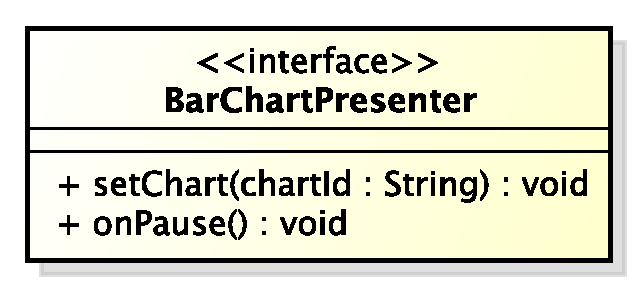
\includegraphics[scale=0.5]{DefinizioneDiProdotto/Pics/Classi/Applicazione--Presenter--BarChartPresenter}
				\caption{Applicazione::Presenter::BarChartPresenter}
			\end{figure}
		}
	
			
			\begin{itemize}
			\item \textbf{Nome:} BarChartPresenter
			\item \textbf{Tipo:} interfaccia
			
		\item \textbf{Estende:}
		Presenter
			\item \textbf{Visibilità:} public
			\item \textbf{Descrizione:} BarChartPresenter è l'interfaccia di BarChartPresenterImpl.
			\item \textbf{Metodi:}
				\begin{itemize}
				\setlength{\itemsep}{5pt}
				
					\item[\ding{111}] {{+setChart(chartId : String) : void}} \\ [1mm] Tale metoto ha il compito di fare a ChartReceiver la richiesta del grafico con un certo id ed aggungersi come osservatore a tale classe in modo tale da esser avvertito qualora il chart sia disponibile.
					\item[\ding{111}] {{+onPause() : void}} \\ [1mm] Tale metodoviene chiamato qualdo l'activity va nello stato di pausa. Esso effettua le operazioni necessarie quando l'activity sta tranditatndo in questo stato. Le operazione qui contenute mireranno quindi al risparmio della batteria come per esempio chiudere il canale socket evitatando quindi che i dati vengano aggiornati inutilmente se l'activity non è in foreground.
				\end{itemize}
		
			\end{itemize}

			
			\level{5}[BarChartPresenterImpl]{Applicazione::Presenter::BarChartPresenterImpl}
			

		\IfFileExists{DefinizioneDiProdotto/Pics/Classi/Applicazione--Presenter--BarChartPresenterImpl.pdf}{
			\begin{figure}[H]
				\centering
				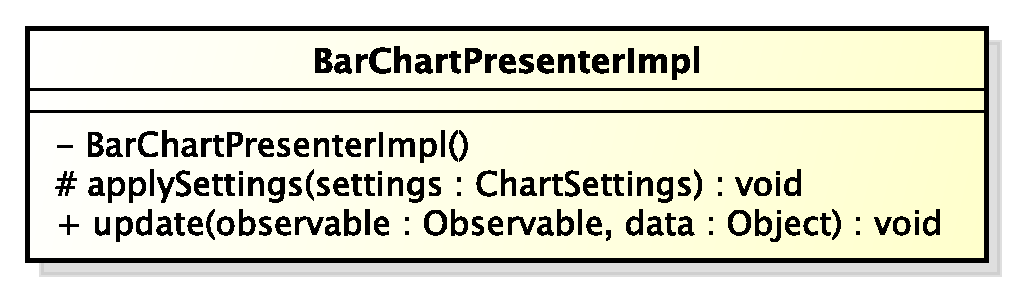
\includegraphics[scale=0.5]{DefinizioneDiProdotto/Pics/Classi/Applicazione--Presenter--BarChartPresenterImpl}
				\caption{Applicazione::Presenter::BarChartPresenterImpl}
			\end{figure}
		}
	
			
			\begin{itemize}
			\item \textbf{Nome:} BarChartPresenterImpl
			\item \textbf{Tipo:} classe
			
		\item \textbf{Estende:}
		ChartPresenterImpl
		\item \textbf{Implementa:}
		BarChartPresenter
		\item \textbf{Astratta:}
		no
			\item \textbf{Visibilità:} package
			\item \textbf{Descrizione:} Tale classe rappresenta l'implementazione di un presenter per table.
			\item \textbf{Metodi:}
				\begin{itemize}
				\setlength{\itemsep}{5pt}
				
					\item[\ding{111}] {{--BarChartPresenterImpl()}} \\ [1mm] Tale metodo è il costruttore. Esso è privato perchè non può esser creata una istanza se non dalla sua classe interna factory.
					\item[\ding{111}] {{\#applySettings(settings : ChartSettings) : void}} \\ [1mm] Tale metodo ha il compito di richiedere alla view la visualizzazione delle varie impostazioni grafiche. Esso dovrà quindi fare una richiesta per ogniuna di tali impostazioni presenti all'interno del parametro settings.
					\item[\ding{111}] {{+update(observable : Observable, data : Object) : void}} \\ [1mm] Tale metodo viene invocato dalla classe osservata qualora siano disponibili i dati del chart richiesto oppure i dati di un aggiornamento. Il parametro observable fa riferimento all'oggetto osservato mentre data contiene un array con i dati utili. Nel caso in cui il dato sia relativo ad un chart tale metodo dovrà creare il chart vero e proprio trasformando precedentemente i vari dati ricevuti (valori e impostazioni) dal formato JSON ad formato necessario ed infine viene richiesto alla view la renderizzazione del chart e l'impostazione delle varie impostazioni grafiche. Nel caso in cui il dato sia riferito ad un aggiornamento dovrà trasformare correttamente tale dato dal formato JSON, aggiornare il modello dei dati utilizzando il metodo di aggiornamento corretto ed infine richiedere alla view la visualizzazione dei nuovi dati.
				\end{itemize}
		
			\end{itemize}

			
			\level{5}[BarChartPresenterFactory]{Applicazione::Presenter::BarChartPresenterImpl::BarChartPresenterFactory}
			

		\IfFileExists{DefinizioneDiProdotto/Pics/Classi/Applicazione--Presenter--BarChartPresenterImpl--BarChartPresenterFactory.pdf}{
			\begin{figure}[H]
				\centering
				\includegraphics[scale=0.5]{DefinizioneDiProdotto/Pics/Classi/Applicazione--Presenter--BarChartPresenterImpl--BarChartPresenterFactory}
				\caption{Applicazione::Presenter::BarChartPresenterImpl::BarChartPresenterFactory}
			\end{figure}
		}
	
			
			\begin{itemize}
			\item \textbf{Nome:} BarChartPresenterFactory
			\item \textbf{Tipo:} classe
			
		\item \textbf{Implementa:}
		PresenterFactory
		\item \textbf{Astratta:}
		no
			\item \textbf{Visibilità:} private
			\item \textbf{Descrizione:} Questa classe si occupa della creazione di un presenter di tipo BarChartPresenterImpl. Tale classe dispone di un blocco di inizializzazione statica che registra la sua istanza nell'Hash map factories della classe PresenterImpl non appena tale classe viene caricata.
			\item \textbf{Attributi:}
				\begin{itemize}
				\setlength{\itemsep}{5pt}
				
					\item[\ding{111}] \underline{--instance : BarChartPresenterFactory} \\ [1mm] Tale attributo statico rappresenta l'istanza univoca di tale classe.
				\end{itemize}
		
			\item \textbf{Metodi:}
				\begin{itemize}
				\setlength{\itemsep}{5pt}
				
					\item[\ding{111}] {\underline{+getInstance() : PresenterFactory}} \\ [1mm] Tale metodo ha il compito di ritornare l'istanza unica di tale classe e se non esiste la crea.
					\item[\ding{111}] {{--BarChartPresenterFactory()}} \\ [1mm] Tale metodo è il costruttore della classe. Esso è privato perchè non si vuole permettere a nessuno di poter creare un'istanza se non utilizzando il metodo getInstance().
					\item[\ding{111}] {{+createPresenter() : PresenterImpl}} \\ [1mm] Tale metodo ha il compito di creare il presenter relativo. Esso può accedere al suo costruttore perchè questa classe factory è interna alla relativa classe presenter. Qualora venga richiesta alla factory la creazione del relativo presenter esso ritornerà l'instanza di quest'ultimo.
				\end{itemize}
		
			\end{itemize}

			
			\level{5}[ChartPresenterImpl]{Applicazione::Presenter::ChartPresenterImpl}
			

		\IfFileExists{DefinizioneDiProdotto/Pics/Classi/Applicazione--Presenter--ChartPresenterImpl.pdf}{
			\begin{figure}[H]
				\centering
				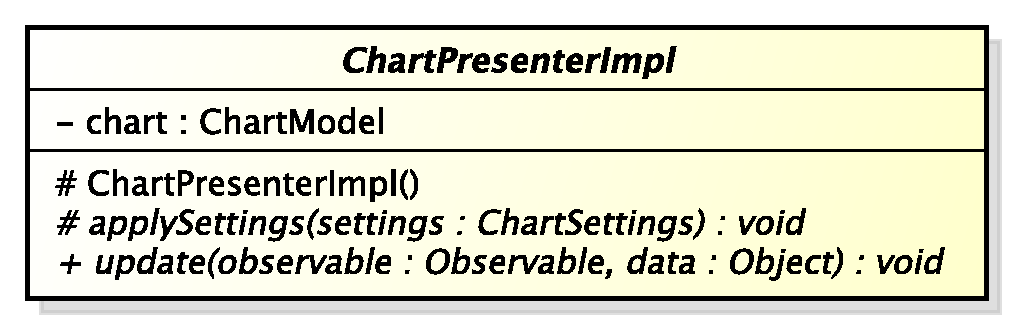
\includegraphics[scale=0.5]{DefinizioneDiProdotto/Pics/Classi/Applicazione--Presenter--ChartPresenterImpl}
				\caption{Applicazione::Presenter::ChartPresenterImpl}
			\end{figure}
		}
	
			
			\begin{itemize}
			\item \textbf{Nome:} ChartPresenterImpl
			\item \textbf{Tipo:} classe
			
		\item \textbf{Estende:}
		PresenterImpl
		\item \textbf{Implementa:}
		Observer
		\item \textbf{Astratta:}
		si
			\item \textbf{Visibilità:} package
			\item \textbf{Descrizione:} Questa classe rappresenta un generico presenter di una vista di un chart. In essa è salvato il riferimento al chart (ChartModel). Tale classe implementa Observer (interfaccia della JDK) con lo scopo di ricevere i dati provenienti dal socket (sfruttando il package Service). Essa infatti può richiedere a ChartUpdater i valori di un grafico oppure richiedere di ricevere i vari aggiornamenti di un certo chart.
			\item \textbf{Attributi:}
				\begin{itemize}
				\setlength{\itemsep}{5pt}
				
					\item[\ding{111}] {--chart : ChartModel} \\ [1mm] Tale attributo rappresenta il riferimento al chart visualizzato nella view
				\end{itemize}
		
			\item \textbf{Metodi:}
				\begin{itemize}
				\setlength{\itemsep}{5pt}
				
					\item[\ding{111}] {{\#ChartPresenterImpl()}} \\ [1mm] Tale metodo è il costuttore della classe. Esso è accessibile solamente alle sottoclassi nella creazione del sottoggetto.
					\item[\ding{111}] \textit{{\#applySettings(settings : ChartSettings) : void}} \\ [1mm] Tale metodo è astratto e definisce un metodo che ha il compito di richiedere alla view la visualizzazione delle varie impostazioni grafiche. Esso dovrà quindi fare una richiesta per ogniuna di tali impostazioni presenti all'interno del parametro settings.
					\item[\ding{111}] \textit{{+update(observable : Observable, data : Object) : void}} \\ [1mm] Tale metodo è astratto e definisce un metodo che quando viene invocato dalla classe osservata qualora siano disponibili i dati del chart richiesto oppure i dati di un aggiornamento. Il parametro observable fa riferimento all'oggetto osservato mentre data contiene un array con i dati utili. Nel caso in cui il dato sia relativo ad un chart tale metodo dovrà creare il chart vero e proprio trasformando precedentemente i vari dati ricevuti (valori e impostazioni) dal formato JSON ad formato necessario ed infine viene richiesto alla view la renderizzazione del chart e l'impostazione delle varie impostazioni grafiche. Nel caso in cui il dato sia riferito ad un aggiornamento dovrà trasformare correttamente tale dato dal formato JSON, aggiornare il modello dei dati utilizzando il metodo di aggiornamento corretto ed infine richiedere alla view la visualizzazione dei nuovi dati.
					\item[\ding{111}] {{+setChart(chartId : String) : void}} \\ [1mm] Tale metoto ha il compito di fare a ChartReceiver la richiesta del grafico con un certo id ed aggungersi come osservatore a tale classe in modo tale da esser avvertito qualora il chart sia disponibile.
					\item[\ding{111}] {{+onPause() : void}} \\ [1mm] Tale metodoviene chiamato qualdo l'activity va nello stato di pausa. Esso effettua le operazioni necessarie quando l'activity sta tranditatndo in questo stato. Le operazione qui contenute mireranno quindi al risparmio della batteria come per esempio chiudere il canale socket evitatando quindi che i dati vengano aggiornati inutilmente se l'activity non è in foreground.
				\end{itemize}
		
			\end{itemize}

			
			\level{5}[HttpRequesterWithCookie]{Applicazione::Presenter::HttpRequesterWithCookie}
			

		\IfFileExists{DefinizioneDiProdotto/Pics/Classi/Applicazione--Presenter--HttpRequesterWithCookie.pdf}{
			\begin{figure}[H]
				\centering
				\includegraphics[scale=0.5]{DefinizioneDiProdotto/Pics/Classi/Applicazione--Presenter--HttpRequesterWithCookie}
				\caption{Applicazione::Presenter::HttpRequesterWithCookie}
			\end{figure}
		}
	
			
			\begin{itemize}
			\item \textbf{Nome:} HttpRequesterWithCookie
			\item \textbf{Tipo:} classe
			
		\item \textbf{Astratta:}
		no
			\item \textbf{Visibilità:} package
			\item \textbf{Descrizione:} Tale classe estende la classe httpClient implementando la possibilità di aggiungere ad eventuali richieste http anche i cookie. Essa ha lo scopo di utilizzare le api esterne di Norris quali autenticazione e richiesta della lista di grafici. Essa salva nel modello le informazioni della sessione.
			\item \textbf{Attributi:}
				\begin{itemize}
				\setlength{\itemsep}{5pt}
				
					\item[\ding{111}] \underline{--instance : HttpRequesterWithCookie} \\ [1mm] Tale attributo statico rappresenta l'istanza univoca di tale classe.
				\end{itemize}
		
			\item \textbf{Metodi:}
				\begin{itemize}
				\setlength{\itemsep}{5pt}
				
					\item[\ding{111}] {\underline{+getInstance() : HttpRequesterWithCookie}} \\ [1mm] Tale metodo ha il compito di ritornare l'istanza unica di tale classe e se non esiste la crea.
					\item[\ding{111}] {{--HttpRequesterWithCookie()}} \\ [1mm] Tale metodo è il costruttore della classe. Esso è privato perchè non si vuole permettere a nessuno di poter creare un'istanza se non chiamando getInstance().
					\item[\ding{111}] {{+getList() : JSONArray}} \\ [1mm] Tale metodo ha il compito di ottenere la lista dei chart presenti nell'istanza di Norris utilizzando le sue Api esterne. Esso dovrà quindi effettuare una richiesta GET verso Norris. I dati necessari per tale richiesta (indirizzo url, endpoint, cookies) sono reperibili in NorrisSessionInfo perchè salvat durante l'operazione di login. Esso Dovrà infine ritornare un Array in formato JSON contente tutti i valori dei vari item della lista.
					\item[\ding{111}] {{+login(addressNorris : String, username : String, password : String) : boolean}} \\ [1mm] Tale metodo ha il compito di effettuare il login all'istanza di Norris richiesta utilizzando le sue Api esterne. I rimanenti due parametri sono le credenziali di autenticazione da utilizzare nel caso in cui la sessione risulti privata. Tale metodo ha il compito di salvare tutti i dati informativi della sessione (indirizzo, endpoint, cookie di autenticazione) per poterli utilizzare qualora necessari. Infine tale metodo ha il compito di sollevare una Exception con il messaggio di errore qualora non sia stato possibile connettersi al server perchè non trovato o per credenziali errate. Il valore ritornato rappresenta l'informazione binaria che dice se è loggato o no.
					\item[\ding{111}] {{+logout() : boolean}} \\ [1mm] Tale metodo ha il compito di effettuare il logout all'istanza di Norris (il cui indirizzo e cookie di autenticazione sono presenti nelle informazioni della sessione salvate nel modello) utilizzando le sue Api esterne. Esso ha il compito di eliminare i dati relativi alla sessione nel modello dei dati qualora il logout abbia avuto successo. Infine esso ritorna l'informazione di avvenuto logout al chiamente.
					\item[\ding{111}] {{+keepAlive() : boolean}} \\ [1mm] Tale metodo ha il compito di tenere attiva la sessione.
					\item[\ding{111}] {{--convertStreamToString(is : InputStream) : String}} \\ [1mm] Tale metodo serve per trasformare gli stream ricevuti dalle richieste get e post della classe in String.
					\item[\ding{111}] {{--makeGetRequest(url : String) : String}} \\ [1mm] Tale metodo permette di effettuare una generica richiesta http di tipo GET ad un certo url passato come parametro. Essa reperisce i cookie di autenticazione nella classe che mantiene le informazioni della sessione.
					\item[\ding{111}] {{--makePostRequestLogin(url : String, params : Map<String,String>, cookieListRef : List<Cookie>) : void}} \\ [1mm] Tale metodo mette permette di effettuare una richiesta http di tipo POST per effettuare il login ad un certo url. I parametri di autenticazioni necessari al server sono custoditi nel parametro params mentre il parametro cookieListRef serve da contenitore per i cookie ricevuti dalla richiesta al server.
					\item[\ding{111}] {{--makePostRequestLogout(url : String) : void}} \\ [1mm] Tale metodo mette permette di effettuare una richiesta http di tipo POST per effettuare il logout ad un certo url. L'unico parametro è quindi l'indirizzo del server a cui fare la richiesta. Essa reperisce i cookie di autenticazione nella classe che mantiene le informazioni della sessione.
				\end{itemize}
		
			\end{itemize}

			
			\level{5}[JSONParser]{Applicazione::Presenter::JSONParser}
			

		\IfFileExists{DefinizioneDiProdotto/Pics/Classi/Applicazione--Presenter--JSONParser.pdf}{
			\begin{figure}[H]
				\centering
				\includegraphics[scale=0.5]{DefinizioneDiProdotto/Pics/Classi/Applicazione--Presenter--JSONParser}
				\caption{Applicazione::Presenter::JSONParser}
			\end{figure}
		}
	
			
			\begin{itemize}
			\item \textbf{Nome:} JSONParser
			\item \textbf{Tipo:} classe
			
		\item \textbf{Astratta:}
		no
			\item \textbf{Visibilità:} package
			\item \textbf{Descrizione:} Questa classe si occupa di fare il parsing dei pacchetti di aggiornamento o di dati di un chart che arrivano dal server in formato JSON.
			\item \textbf{Attributi:}
				\begin{itemize}
				\setlength{\itemsep}{5pt}
				
					\item[\ding{111}] \underline{--instance : JSONParser} \\ [1mm] Tale attributo statico rappresenta l'istanza univoca di tale classe.
				\end{itemize}
		
			\item \textbf{Metodi:}
				\begin{itemize}
				\setlength{\itemsep}{5pt}
				
					\item[\ding{111}] {\underline{+getInstance() : JSONParser}} \\ [1mm] Tale metodo statico viene chiamato per ricevere l'istanza univoca per la classe.
					\item[\ding{111}] {{--JSONParser()}} \\ [1mm] Rappresenta il costruttore di JSONParser. Esso è privato perchè lo si vuole nascondere all'esterno, costringendo a sfruttare il design pattern singleton attraverso il metodo getInstance().
					\item[\ding{111}] {{+parseBarChart(chartData : JSONObject) : ChartData}} \\ [1mm] Tale metodo permette di trasformare i dati di un Bar Chart dal formato JSON a ChartData ed ovviamente con tipo dinamico BarChartData.
					\item[\ding{111}] {{+parseLineChart(chartData : JSONObject) : ChartData}} \\ [1mm] Tale metodo permette di trasformare i dati di un Line Chart dal formato JSON a ChartData ed ovviamente con tipo dinamico LineChartData.
					\item[\ding{111}] {{+parseMapChart(chartData : JSONObject) : ChartData}} \\ [1mm] Tale metodo permette di trasformare i dati di un Map Chart dal formato JSON a ChartData ed ovviamente con tipo dinamico MapChartData.
					\item[\ding{111}] {{+parseTable(chartData : JSONObject) : ChartData}} \\ [1mm] Tale metodo permette di trasformare i dati di una Table dal formato JSON a ChartData ed ovviamente con tipo dinamico TableData.
					\item[\ding{111}] {{+parseBarChartSettings(chartSettinsg : JSONObject) : ChartSettings}} \\ [1mm] Tale metodo permette di trasformare le impostazioni di un bar chart dal formato JSON a ChartSettings. il tipo dinamico ritornato sarà dunque BarChartSettingsImpl.
					\item[\ding{111}] {{+parseLineChartSettings(chartSettinsg : JSONObject) : ChartSettings}} \\ [1mm] Tale metodo permette di trasformare le impostazioni di un line chart dal formato JSON a ChartSettings. il tipo dinamico ritornato sarà dunque LineChartSettingsImpl.
					\item[\ding{111}] {{+parseMapChartSettings(chartSettinsg : JSONObject) : ChartSettings}} \\ [1mm] Tale metodo permette di trasformare le impostazioni di un map chart dal formato JSON a ChartSettings. il tipo dinamico ritornato sarà dunque MapChartSettingsImpl.
					\item[\ding{111}] {{+parseTableSettings(chartSettinsg : JSONObject) : ChartSettings}} \\ [1mm] Tale metodo permette di trasformare le impostazioni di una table dal formato JSON a ChartSettings. il tipo dinamico ritornato sarà dunque TableSettingsImpl.
					\item[\ding{111}] {{+parseBarChartInPlaceUpdate(updateData : JSONObject) : ChartUpdate}} \\ [1mm] Tale metodo permette di trasformare un aggiornamento in place di un bar chart dal formato JSON a ChartUpdate. Il tipo dinamico di tale oggetto ritornato sarà dunque di tipo dinamico BarChartInPlaceUpdate.
					\item[\ding{111}] {{+parseLineChartInPlaceUpdate(updateData : JSONObject) : ChartUpdate}} \\ [1mm] Tale metodo permette di trasformare un aggiornamento in place di un line chart dal formato JSON a ChartUpdate. Il tipo dinamico di tale oggetto ritornato sarà dunque di tipo dinamico LineChartInPlaceUpdate.
					\item[\ding{111}] {{+parseLineChartStreamUpdate(updateData : JSONObject) : ChartUpdate}} \\ [1mm] Tale metodo permette di trasformare un aggiornamento stream di un line chart dal formato JSON a ChartUpdate. Il tipo dinamico di tale oggetto ritornato sarà dunque di tipo dinamico LineChartStreamUpdate.
					\item[\ding{111}] {{+parseMapChartInPlaceUpdate(updateData : JSONObject) : ChartUpdate}} \\ [1mm] Tale metodo permette di trasformare un aggiornamento in place di un map chart dal formato JSON a ChartUpdate. Il tipo dinamico di tale oggetto ritornato sarà dunque di tipo dinamico MapChartInPlaceUpdate.
					\item[\ding{111}] {{+parseMapChartMovieUpdate(updateData : JSONObject) : ChartUpdate}} \\ [1mm] Tale metodo permette di trasformare un aggiornamento movie di un map chart dal formato JSON a ChartUpdate. Il tipo dinamico di tale oggetto ritornato sarà dunque di tipo dinamico MapChartMovieUpdate.
Tale metodo utilizzerà i metodi parseMapChartDeleteUpdate, parseMapChartStreamUpdate e parseMapChartInPlaceUpdate per trasformare tutte le sue parti.
					\item[\ding{111}] {{--parseMapChartDeleteUpdate(updateData : JSONObject) : ChartUpdate}} \\ [1mm] Tale metodo permette di trasformare un pacchetto delete di un map chart dal formato JSON a ChartUpdate. Il tipo dinamico di tale oggetto ritornato sarà dunque di tipo dinamico MapChartDeleteUpdate.
Tale metodo è privato perchè serve al metodo parseMapChartMovieUpdate per trasformare il pacchetto delete dell'aggiornamento movie.
					\item[\ding{111}] {{--parseMapChartStreamUpdate(updateData : JSONObject) : ChartUpdate}} \\ [1mm] Tale metodo permette di trasformare un aggiornamento stream di un map chart dal formato JSON a ChartUpdate. Il tipo dinamico di tale oggetto ritornato sarà dunque di tipo dinamico MapChartStreamUpdate.
Tale metodo è privato perchè serve al metodo parseMapChartMovieUpdate per trasformare il pacchetto stream dell'aggiornamento movie.
					\item[\ding{111}] {{+parseTableInPlaceUpdate(updateData : JSONObject) : ChartUpdate}} \\ [1mm] Tale metodo permette di trasformare un aggiornamento in place di una table dal formato JSON a ChartUpdate. Il tipo dinamico di tale oggetto ritornato sarà dunque di tipo dinamico TableStreamUpdate.
					\item[\ding{111}] {{+parseTableStreamUpdate(updateData : JSONObject) : ChartUpdate}} \\ [1mm] Tale metodo permette di trasformare un aggiornamento stream di una table dal formato JSON a ChartUpdate. Il tipo dinamico di tale oggetto ritornato sarà dunque di tipo dinamico TableStreamUpdate.
				\end{itemize}
		
			\end{itemize}

			
			\level{5}[LineChartPresenter]{Applicazione::Presenter::LineChartPresenter}
			

		\IfFileExists{DefinizioneDiProdotto/Pics/Classi/Applicazione--Presenter--LineChartPresenter.pdf}{
			\begin{figure}[H]
				\centering
				\includegraphics[scale=0.5]{DefinizioneDiProdotto/Pics/Classi/Applicazione--Presenter--LineChartPresenter}
				\caption{Applicazione::Presenter::LineChartPresenter}
			\end{figure}
		}
	
			
			\begin{itemize}
			\item \textbf{Nome:} LineChartPresenter
			\item \textbf{Tipo:} interfaccia
			
		\item \textbf{Estende:}
		Presenter
			\item \textbf{Visibilità:} public
			\item \textbf{Descrizione:} LinaChartPresenter è l'interfaccia di LineChartPresenterImpl.
			\item \textbf{Metodi:}
				\begin{itemize}
				\setlength{\itemsep}{5pt}
				
					\item[\ding{111}] {{+setChart(chartId : String) : void}} \\ [1mm] Tale metoto ha il compito di fare a ChartReceiver la richiesta del grafico con un certo id ed aggungersi come osservatore a tale classe in modo tale da esser avvertito qualora il chart sia disponibile.
					\item[\ding{111}] {{+onPause() : void}} \\ [1mm] Tale metodoviene chiamato qualdo l'activity va nello stato di pausa. Esso effettua le operazioni necessarie quando l'activity sta tranditatndo in questo stato. Le operazione qui contenute mireranno quindi al risparmio della batteria come per esempio chiudere il canale socket evitatando quindi che i dati vengano aggiornati inutilmente se l'activity non è in foreground.
				\end{itemize}
		
			\end{itemize}

			
			\level{5}[LineChartPresenterImpl]{Applicazione::Presenter::LineChartPresenterImpl}
			

		\IfFileExists{DefinizioneDiProdotto/Pics/Classi/Applicazione--Presenter--LineChartPresenterImpl.pdf}{
			\begin{figure}[H]
				\centering
				\includegraphics[scale=0.5]{DefinizioneDiProdotto/Pics/Classi/Applicazione--Presenter--LineChartPresenterImpl}
				\caption{Applicazione::Presenter::LineChartPresenterImpl}
			\end{figure}
		}
	
			
			\begin{itemize}
			\item \textbf{Nome:} LineChartPresenterImpl
			\item \textbf{Tipo:} classe
			
		\item \textbf{Estende:}
		ChartPresenterImpl
		\item \textbf{Implementa:}
		LineChartPresenter
		\item \textbf{Astratta:}
		no
			\item \textbf{Visibilità:} package
			\item \textbf{Descrizione:} Tale classe rappresenta l'implementazione di un presenter per line chart.
			\item \textbf{Metodi:}
				\begin{itemize}
				\setlength{\itemsep}{5pt}
				
					\item[\ding{111}] {{--LineChartPresenterImpl()}} \\ [1mm] Tale metodo è il costruttore. Esso è privato perchè non può esser creata una istanza se non dalla sua classe interna factory.
					\item[\ding{111}] {{+update(observable : Observable, data : Object) : void}} \\ [1mm] Tale metodo viene invocato dalla classe osservata qualora siano disponibili i dati del chart richiesto oppure i dati di un aggiornamento. Il parametro observable fa riferimento all'oggetto osservato mentre data contiene un array con i dati utili. Nel caso in cui il dato sia relativo ad un chart tale metodo dovrà creare il chart vero e proprio trasformando precedentemente i vari dati ricevuti (valori e impostazioni) dal formato JSON ad formato necessario ed infine viene richiesto alla view la renderizzazione del chart e l'impostazione delle varie impostazioni grafiche. Nel caso in cui il dato sia riferito ad un aggiornamento dovrà trasformare correttamente tale dato dal formato JSON, aggiornare il modello dei dati utilizzando il metodo di aggiornamento corretto ed infine richiedere alla view la visualizzazione dei nuovi dati.
					\item[\ding{111}] {{\#applySettings(settings : ChartSettings) : void}} \\ [1mm] Tale metodo ha il compito di richiedere alla view la visualizzazione delle varie impostazioni grafiche. Esso dovrà quindi fare una richiesta per ogniuna di tali impostazioni presenti all'interno del parametro settings.
				\end{itemize}
		
			\end{itemize}

			
			\level{5}[LineChartPresenterFactory]{Applicazione::Presenter::LineChartPresenterImpl::LineChartPresenterFactory}
			

		\IfFileExists{DefinizioneDiProdotto/Pics/Classi/Applicazione--Presenter--LineChartPresenterImpl--LineChartPresenterFactory.pdf}{
			\begin{figure}[H]
				\centering
				\includegraphics[scale=0.5]{DefinizioneDiProdotto/Pics/Classi/Applicazione--Presenter--LineChartPresenterImpl--LineChartPresenterFactory}
				\caption{Applicazione::Presenter::LineChartPresenterImpl::LineChartPresenterFactory}
			\end{figure}
		}
	
			
			\begin{itemize}
			\item \textbf{Nome:} LineChartPresenterFactory
			\item \textbf{Tipo:} classe
			
		\item \textbf{Implementa:}
		PresenterFactory
		\item \textbf{Astratta:}
		no
			\item \textbf{Visibilità:} private
			\item \textbf{Descrizione:} Questa classe si occupa della creazione di un presenter di tipo LineChartPresenterImpl. Tale classe dispone di un blocco di inizializzazione statica che registra la sua istanza nell'Hash map factories della classe PresenterImpl non appena tale classe viene caricata.
			\item \textbf{Attributi:}
				\begin{itemize}
				\setlength{\itemsep}{5pt}
				
					\item[\ding{111}] \underline{--instance : LineChartPresenterFactory} \\ [1mm] Tale attributo statico rappresenta l'istanza univoca di tale classe.
				\end{itemize}
		
			\item \textbf{Metodi:}
				\begin{itemize}
				\setlength{\itemsep}{5pt}
				
					\item[\ding{111}] {\underline{+getInstance() : PresenterFactory}} \\ [1mm] Tale metodo ha il compito di ritornare l'istanza unica di tale classe e se non esiste la crea.
					\item[\ding{111}] {{--LineChartPresenterFactory()}} \\ [1mm] Tale metodo è il costruttore della classe. Esso è privato perchè non si vuole permettere a nessuno di poter creare un'istanza se non utilizzando il metodo getInstance().
					\item[\ding{111}] {{+createPresenter() : PresenterImpl}} \\ [1mm] Tale metodo ha il compito di creare il presenter relativo. Esso può accedere al suo costruttore perchè questa classe factory è interna alla relativa classe presenter. Qualora venga richiesta alla factory la creazione del relativo presenter esso ritornerà l'instanza di quest'ultimo.
				\end{itemize}
		
			\end{itemize}

			
			\level{5}[ListPresenter]{Applicazione::Presenter::ListPresenter}
			

		\IfFileExists{DefinizioneDiProdotto/Pics/Classi/Applicazione--Presenter--ListPresenter.pdf}{
			\begin{figure}[H]
				\centering
				\includegraphics[scale=0.5]{DefinizioneDiProdotto/Pics/Classi/Applicazione--Presenter--ListPresenter}
				\caption{Applicazione::Presenter::ListPresenter}
			\end{figure}
		}
	
			
			\begin{itemize}
			\item \textbf{Nome:} ListPresenter
			\item \textbf{Tipo:} interfaccia
			
		\item \textbf{Estende:}
		Presenter
			\item \textbf{Visibilità:} public
			\item \textbf{Descrizione:} ListPresenter è l'interfaccia di ListPresenterImpl.
			\item \textbf{Metodi:}
				\begin{itemize}
				\setlength{\itemsep}{5pt}
				
					\item[\ding{111}] {{+onResume() : void}} \\ [1mm] Tale metodo viene invocato in risposta ad un evento nella view, ovvero la visualizzazione dell'activity con la lista dei chart. Esso ha il compito di ottenere la lista (attraverso HttpRequesterWithCookie) e modificare la view con tali valori.
					\item[\ding{111}] {{+onItemClicked(chartType : String, chartId : String) : void}} \\ [1mm] Tale metodo viene invocato alla pressione di un elemento della lista. Esso chiederà la visualizzazione della chartActivity specifica del chart rappresentato nell'elemento.
					\item[\ding{111}] {{+onLogoutClick() : void}} \\ [1mm] Tale metodo viene invocato alla pressione del bottone di logout nella view. Esso effettuerà il logout dalla sessione (attraverso HttpRequesterWithCookie).
				\end{itemize}
		
			\end{itemize}

			
			\level{5}[ListPresenterImpl]{Applicazione::Presenter::ListPresenterImpl}
			

		\IfFileExists{DefinizioneDiProdotto/Pics/Classi/Applicazione--Presenter--ListPresenterImpl.pdf}{
			\begin{figure}[H]
				\centering
				\includegraphics[scale=0.5]{DefinizioneDiProdotto/Pics/Classi/Applicazione--Presenter--ListPresenterImpl}
				\caption{Applicazione::Presenter::ListPresenterImpl}
			\end{figure}
		}
	
			
			\begin{itemize}
			\item \textbf{Nome:} ListPresenterImpl
			\item \textbf{Tipo:} classe
			
		\item \textbf{Estende:}
		PresenterImpl
		\item \textbf{Implementa:}
		ListPresenter
		\item \textbf{Astratta:}
		no
			\item \textbf{Visibilità:} package
			\item \textbf{Descrizione:} Questa classe rappresenta la specializzazione di PresenterImpl. Essa ha lo scopo di modificare la View della lista dei grafici presenti all'interno dell'istanza di Norris e quindi richiedere ad HttpRequesterWithCookie la lista di chart presenti all'interno dell'istanza. Tale classe infine permette di effettuare il logout della sessione attiva.
			\item \textbf{Metodi:}
				\begin{itemize}
				\setlength{\itemsep}{5pt}
				
					\item[\ding{111}] {{--ListPresenterImpl()}} \\ [1mm] Tale metodo è il costruttore. Esso è privato perchè non può esser creata una istanza se non dalla sua classe interna factory.
					\item[\ding{111}] {{+onResume() : void}} \\ [1mm] Tale metodo viene invocato in risposta ad un evento nella view, ovvero la visualizzazione dell'activity con la lista dei chart. Esso ha il compito di ottenere la lista (attraverso HttpRequesterWithCookie) e modificare la view con tali valori.
					\item[\ding{111}] {{+onItemClicked(chartType : String, chartId : String) : void}} \\ [1mm] Tale metodo viene invocato alla pressione di un elemento della lista. Esso chiederà la visualizzazione della chartActivity specifica del chart rappresentato nell'elemento. Esso dovrà passare i dati relativi a quale chart si vuole visualizzare.
					\item[\ding{111}] {{+onLogoutClick() : void}} \\ [1mm] Tale metodo viene invocato alla pressione del bottone di logout nella view. Utilzzando la classe HttpRequesterWithCookie effettuerà il logout.
				\end{itemize}
		
			\end{itemize}

			
			\level{5}[ListPresenterFactory]{Applicazione::Presenter::ListPresenterImpl::ListPresenterFactory}
			

		\IfFileExists{DefinizioneDiProdotto/Pics/Classi/Applicazione--Presenter--ListPresenterImpl--ListPresenterFactory.pdf}{
			\begin{figure}[H]
				\centering
				\includegraphics[scale=0.5]{DefinizioneDiProdotto/Pics/Classi/Applicazione--Presenter--ListPresenterImpl--ListPresenterFactory}
				\caption{Applicazione::Presenter::ListPresenterImpl::ListPresenterFactory}
			\end{figure}
		}
	
			
			\begin{itemize}
			\item \textbf{Nome:} ListPresenterFactory
			\item \textbf{Tipo:} classe
			
		\item \textbf{Implementa:}
		PresenterFactory
		\item \textbf{Astratta:}
		no
			\item \textbf{Visibilità:} private
			\item \textbf{Descrizione:} Questa classe si occupa della creazione di un presenter di tipo ListPresenterImpl.  Tale classe dispone di un blocco di inizializzazione statica che registra la sua istanza nell'Hash map factories della classe PresenterImpl non appena tale classe viene caricata.
			\item \textbf{Attributi:}
				\begin{itemize}
				\setlength{\itemsep}{5pt}
				
					\item[\ding{111}] \underline{--instance : ListPresenterFactory} \\ [1mm] Tale attributo statico rappresenta l'istanza univoca di tale classe.
				\end{itemize}
		
			\item \textbf{Metodi:}
				\begin{itemize}
				\setlength{\itemsep}{5pt}
				
					\item[\ding{111}] {\underline{+getInstance() : PresenterFactory}} \\ [1mm] Tale metodo ha il compito di ritornare l'istanza unica di tale classe e se non esiste la crea.
					\item[\ding{111}] {{--ListPresenterFactory()}} \\ [1mm] Tale metodo è il costruttore della classe. Esso è privato perchè non si vuole permettere a nessuno di poter creare un'istanza se non utilizzando il metodo getInstance().
					\item[\ding{111}] {{+createPresenter() : PresenterImpl}} \\ [1mm] Tale metodo ha il compito di creare il presenter relativo. Esso può accedere al suo costruttore perchè questa classe factory è interna alla relativa classe presenter. Qualora venga richiesta alla factory la creazione del relativo presenter esso ritornerà l'instanza di quest'ultimo.
				\end{itemize}
		
			\end{itemize}

			
			\level{5}[LoginPresenter]{Applicazione::Presenter::LoginPresenter}
			

		\IfFileExists{DefinizioneDiProdotto/Pics/Classi/Applicazione--Presenter--LoginPresenter.pdf}{
			\begin{figure}[H]
				\centering
				\includegraphics[scale=0.5]{DefinizioneDiProdotto/Pics/Classi/Applicazione--Presenter--LoginPresenter}
				\caption{Applicazione::Presenter::LoginPresenter}
			\end{figure}
		}
	
			
			\begin{itemize}
			\item \textbf{Nome:} LoginPresenter
			\item \textbf{Tipo:} interfaccia
			
		\item \textbf{Estende:}
		Presenter
			\item \textbf{Visibilità:} public
			\item \textbf{Descrizione:} LoginPresenter è l'interfaccia di LoginPresenterImpl.
			\item \textbf{Metodi:}
				\begin{itemize}
				\setlength{\itemsep}{5pt}
				
					\item[\ding{111}] {{+onLoginClick(addressNorris : String, username : String, password : String) : boolean}} \\ [1mm] Tale metodo gestisce la user gesture di un click sul bottone di login nella view. Esso tenterà di effettuare il login mettendo il segnale di attesa sulla view e se questo ha successo viene mostrata la view con la lista dei chart altrimenti viene visualizzato sulla view un messaggio di errore.
				\end{itemize}
		
			\end{itemize}

			
			\level{5}[LoginPresenterImpl]{Applicazione::Presenter::LoginPresenterImpl}
			

		\IfFileExists{DefinizioneDiProdotto/Pics/Classi/Applicazione--Presenter--LoginPresenterImpl.pdf}{
			\begin{figure}[H]
				\centering
				\includegraphics[scale=0.5]{DefinizioneDiProdotto/Pics/Classi/Applicazione--Presenter--LoginPresenterImpl}
				\caption{Applicazione::Presenter::LoginPresenterImpl}
			\end{figure}
		}
	
			
			\begin{itemize}
			\item \textbf{Nome:} LoginPresenterImpl
			\item \textbf{Tipo:} classe
			
		\item \textbf{Estende:}
		PresenterImpl
		\item \textbf{Implementa:}
		LoginPresenter
		\item \textbf{Astratta:}
		no
			\item \textbf{Visibilità:} package
			\item \textbf{Descrizione:} Questa classe rappresenta la specializzazione di PresenterImpl. Essa ha lo scopo di modificare la View della della home. Ha il compito di richiedere ad HttpRequesterWithCookie l'accesso ad una istanza di Norris attraverso login.
			\item \textbf{Metodi:}
				\begin{itemize}
				\setlength{\itemsep}{5pt}
				
					\item[\ding{111}] {{--LoginPresenterImpl()}} \\ [1mm] Tale metodo è il costruttore. Esso è privato perchè non può esser creata una istanza se non dalla sua classe interna factory.
					\item[\ding{111}] {{+onLoginClick(addressNorris : String, username : String, password : String) : void}} \\ [1mm] Tale metodo gestisce la user gesture di un click sul bottone di login nella view. Esso tenterà di effettuare il login mettendo il segnale di attesa sulla view e se questo ha successo viene mostrata la view con la lista dei chart altrimenti viene visualizzato sulla view un messaggio di errore.
				\end{itemize}
		
			\end{itemize}

			
			\level{5}[LoginPresenterFactory]{Applicazione::Presenter::LoginPresenterImpl::LoginPresenterFactory}
			

		\IfFileExists{DefinizioneDiProdotto/Pics/Classi/Applicazione--Presenter--LoginPresenterImpl--LoginPresenterFactory.pdf}{
			\begin{figure}[H]
				\centering
				\includegraphics[scale=0.5]{DefinizioneDiProdotto/Pics/Classi/Applicazione--Presenter--LoginPresenterImpl--LoginPresenterFactory}
				\caption{Applicazione::Presenter::LoginPresenterImpl::LoginPresenterFactory}
			\end{figure}
		}
	
			
			\begin{itemize}
			\item \textbf{Nome:} LoginPresenterFactory
			\item \textbf{Tipo:} classe
			
		\item \textbf{Implementa:}
		PresenterFactory
		\item \textbf{Astratta:}
		no
			\item \textbf{Visibilità:} private
			\item \textbf{Descrizione:} Questa classe si occupa della creazione di un presenter di tipo LoginPresenterImpl.  Tale classe dispone di un blocco di inizializzazione statica che registra la sua istanza nell'Hash map factories della classe PresenterImpl non appena tale classe viene caricata.
			\item \textbf{Attributi:}
				\begin{itemize}
				\setlength{\itemsep}{5pt}
				
					\item[\ding{111}] \underline{--instance : LoginPresenterFactory} \\ [1mm] Tale attributo statico rappresenta l'istanza univoca di tale classe.
				\end{itemize}
		
			\item \textbf{Metodi:}
				\begin{itemize}
				\setlength{\itemsep}{5pt}
				
					\item[\ding{111}] {\underline{+getInstance() : PresenterFactory}} \\ [1mm] Tale metodo ha il compito di ritornare l'istanza unica di tale classe e se non esiste la crea.
					\item[\ding{111}] {{--LoginPresenterFactory()}} \\ [1mm] Tale metodo è il costruttore della classe. Esso è privato perchè non si vuole permettere a nessuno di poter creare un'istanza se non utilizzando il metodo getInstance().
					\item[\ding{111}] {{+createPresenter() : PresenterImpl}} \\ [1mm] Tale metodo ha il compito di creare il presenter relativo. Esso può accedere al suo costruttore perchè questa classe factory è interna alla relativa classe presenter. Qualora venga richiesta alla factory la creazione del relativo presenter esso ritornerà l'instanza di quest'ultimo.
				\end{itemize}
		
			\end{itemize}

			
			\level{5}[MapChartPresenter]{Applicazione::Presenter::MapChartPresenter}
			

		\IfFileExists{DefinizioneDiProdotto/Pics/Classi/Applicazione--Presenter--MapChartPresenter.pdf}{
			\begin{figure}[H]
				\centering
				\includegraphics[scale=0.5]{DefinizioneDiProdotto/Pics/Classi/Applicazione--Presenter--MapChartPresenter}
				\caption{Applicazione::Presenter::MapChartPresenter}
			\end{figure}
		}
	
			
			\begin{itemize}
			\item \textbf{Nome:} MapChartPresenter
			\item \textbf{Tipo:} interfaccia
			
		\item \textbf{Estende:}
		Presenter
			\item \textbf{Visibilità:} public
			\item \textbf{Descrizione:} MapChartPresenter è l'interfaccia di MapChartPresenterImpl.
			\item \textbf{Metodi:}
				\begin{itemize}
				\setlength{\itemsep}{5pt}
				
					\item[\ding{111}] {{+setChart(chartId : String) : void}} \\ [1mm] Tale metoto ha il compito di fare a ChartReceiver la richiesta del grafico con un certo id ed aggungersi come osservatore a tale classe in modo tale da esser avvertito qualora il chart sia disponibile.
					\item[\ding{111}] {{+onPause() : void}} \\ [1mm] Tale metodoviene chiamato qualdo l'activity va nello stato di pausa. Esso effettua le operazioni necessarie quando l'activity sta tranditatndo in questo stato. Le operazione qui contenute mireranno quindi al risparmio della batteria come per esempio chiudere il canale socket evitatando quindi che i dati vengano aggiornati inutilmente se l'activity non è in foreground.
				\end{itemize}
		
			\end{itemize}

			
			\level{5}[MapChartPresenterImpl]{Applicazione::Presenter::MapChartPresenterImpl}
			

		\IfFileExists{DefinizioneDiProdotto/Pics/Classi/Applicazione--Presenter--MapChartPresenterImpl.pdf}{
			\begin{figure}[H]
				\centering
				\includegraphics[scale=0.5]{DefinizioneDiProdotto/Pics/Classi/Applicazione--Presenter--MapChartPresenterImpl}
				\caption{Applicazione::Presenter::MapChartPresenterImpl}
			\end{figure}
		}
	
			
			\begin{itemize}
			\item \textbf{Nome:} MapChartPresenterImpl
			\item \textbf{Tipo:} classe
			
		\item \textbf{Estende:}
		ChartPresenterImpl
		\item \textbf{Implementa:}
		MapChartPresenter
		\item \textbf{Astratta:}
		no
			\item \textbf{Visibilità:} package
			\item \textbf{Descrizione:} Tale classe rappresenta l'implementazione di un presenter per table.
			\item \textbf{Metodi:}
				\begin{itemize}
				\setlength{\itemsep}{5pt}
				
					\item[\ding{111}] {{--MapChartPresenterImpl()}} \\ [1mm] Tale metodo è il costruttore. Esso è privato perchè non può esser creata una istanza se non dalla sua classe interna factory.
					\item[\ding{111}] {{\#applySettings(settings : ChartSettings) : void}} \\ [1mm] Tale metodo ha il compito di richiedere alla view la visualizzazione delle varie impostazioni grafiche. Esso dovrà quindi fare una richiesta per ogniuna di tali impostazioni presenti all'interno del parametro settings.
					\item[\ding{111}] {{+update(observable : Observable, data : Object) : void}} \\ [1mm] Tale metodo viene invocato dalla classe osservata qualora siano disponibili i dati del chart richiesto oppure i dati di un aggiornamento. Il parametro observable fa riferimento all'oggetto osservato mentre data contiene un array con i dati utili. Nel caso in cui il dato sia relativo ad un chart tale metodo dovrà creare il chart vero e proprio trasformando precedentemente i vari dati ricevuti (valori e impostazioni) dal formato JSON ad formato necessario ed infine viene richiesto alla view la renderizzazione del chart e l'impostazione delle varie impostazioni grafiche. Nel caso in cui il dato sia riferito ad un aggiornamento dovrà trasformare correttamente tale dato dal formato JSON, aggiornare il modello dei dati utilizzando il metodo di aggiornamento corretto ed infine richiedere alla view la visualizzazione dei nuovi dati.
				\end{itemize}
		
			\end{itemize}

			
			\level{5}[MapChartPresenterFactory]{Applicazione::Presenter::MapChartPresenterImpl::MapChartPresenterFactory}
			

		\IfFileExists{DefinizioneDiProdotto/Pics/Classi/Applicazione--Presenter--MapChartPresenterImpl--MapChartPresenterFactory.pdf}{
			\begin{figure}[H]
				\centering
				\includegraphics[scale=0.5]{DefinizioneDiProdotto/Pics/Classi/Applicazione--Presenter--MapChartPresenterImpl--MapChartPresenterFactory}
				\caption{Applicazione::Presenter::MapChartPresenterImpl::MapChartPresenterFactory}
			\end{figure}
		}
	
			
			\begin{itemize}
			\item \textbf{Nome:} MapChartPresenterFactory
			\item \textbf{Tipo:} classe
			
		\item \textbf{Implementa:}
		PresenterFactory
		\item \textbf{Astratta:}
		no
			\item \textbf{Visibilità:} private
			\item \textbf{Descrizione:} Questa classe si occupa della creazione di un presenter di tipo MapChartPresenterImpl. Tale classe dispone di un blocco di inizializzazione statica che registra la sua istanza nell'Hash map factories della classe PresenterImpl non appena tale classe viene caricata.
			\item \textbf{Attributi:}
				\begin{itemize}
				\setlength{\itemsep}{5pt}
				
					\item[\ding{111}] \underline{--instance : MapChartPresenterFactory} \\ [1mm] Tale attributo statico rappresenta l'istanza univoca di tale classe.
				\end{itemize}
		
			\item \textbf{Metodi:}
				\begin{itemize}
				\setlength{\itemsep}{5pt}
				
					\item[\ding{111}] {\underline{+getInstance() : PresenterFactory}} \\ [1mm] Tale metodo ha il compito di ritornare l'istanza unica di tale classe e se non esiste la crea.
					\item[\ding{111}] {{--MapChartPresenterFactory()}} \\ [1mm] Tale metodo è il costruttore della classe. Esso è privato perchè non si vuole permettere a nessuno di poter creare un'istanza se non utilizzando il metodo getInstance().
					\item[\ding{111}] {{+createPresenter() : PresenterImpl}} \\ [1mm] Tale metodo ha il compito di creare il presenter relativo. Esso può accedere al suo costruttore perchè questa classe factory è interna alla relativa classe presenter. Qualora venga richiesta alla factory la creazione del relativo presenter esso ritornerà l'instanza di quest'ultimo.
				\end{itemize}
		
			\end{itemize}

			
			\level{5}[Presenter]{Applicazione::Presenter::Presenter}
			

		\IfFileExists{DefinizioneDiProdotto/Pics/Classi/Applicazione--Presenter--Presenter.pdf}{
			\begin{figure}[H]
				\centering
				\includegraphics[scale=0.5]{DefinizioneDiProdotto/Pics/Classi/Applicazione--Presenter--Presenter}
				\caption{Applicazione::Presenter::Presenter}
			\end{figure}
		}
	
			
			\begin{itemize}
			\item \textbf{Nome:} Presenter
			\item \textbf{Tipo:} interfaccia
			
			\item \textbf{Visibilità:} public
			\item \textbf{Descrizione:} LoginPresenter è l'interfaccia che rappresenta un qualsiasi presenter.
			\end{itemize}

			
			\level{5}[PresenterImpl]{Applicazione::Presenter::PresenterImpl}
			

		\IfFileExists{DefinizioneDiProdotto/Pics/Classi/Applicazione--Presenter--PresenterImpl.pdf}{
			\begin{figure}[H]
				\centering
				\includegraphics[scale=0.5]{DefinizioneDiProdotto/Pics/Classi/Applicazione--Presenter--PresenterImpl}
				\caption{Applicazione::Presenter::PresenterImpl}
			\end{figure}
		}
	
			
			\begin{itemize}
			\item \textbf{Nome:} PresenterImpl
			\item \textbf{Tipo:} classe
			
		\item \textbf{Implementa:}
		Presenter
		\item \textbf{Astratta:}
		si
			\item \textbf{Visibilità:} public
			\item \textbf{Descrizione:} Questa classe rappresenta un presenter generico e per questo motivo è una classe astratta. Essa contiene al suo interno il riferimento alla view a cui è associato. Contiene, inoltre, la interfaccia PresenterFactory e un hashmap che si occupa della corrispondenza tra le tipologie di presenter e le rispettive classi factory. La classe contiene delle costanti statiche che servono per identificare le varie tipologie di presenter.
			\item \textbf{Attributi:}
				\begin{itemize}
				\setlength{\itemsep}{5pt}
				
					\item[\ding{111}] \underline{--factories : Map<PresenterType,PresenterFactory>} \\ [1mm] Tale hashmap contiene le associazioni di tutti i tipi di presenter possibilli con la relativa factory dei presenter.
					\item[\ding{111}] {\#view : View} \\ [1mm] Tale attributo rappresenta il riferimento alla view relativa al presenter.
					\item[\ding{111}] {+PresenterType : Enum} \\ [1mm] Contiene i tipi di presenter contenuti nell'HashMap factories.
				\end{itemize}
		
			\item \textbf{Metodi:}
				\begin{itemize}
				\setlength{\itemsep}{5pt}
				
					\item[\ding{111}] {\underline{\#registerFactory(presenterType : PresenterType, factory : PresenterFactory) : void}} \\ [1mm] Tale metodo serve per registrare una certa factory al relativo presenter nell'hashmap della classe.
					\item[\ding{111}] {\underline{+create(presenterType : PresenterType, view : View) : Presenter}} \\ [1mm] Tale metodo non fa altro che creare il presenter associato al parametro presenterType, inizializzare il campo relativo alla view con il parametro view ed infine ritornare l'interfaccia Presenter di tale istanza creata.
					\item[\ding{111}] {{\#PresenterImpl(view : View) : void}} \\ [1mm] Tale metodo è il costruttore della classe. Esso è protected perchè non si vuole permettere a classi non autorizzate di creare direttamente un'istanza di tale classe.
				\end{itemize}
		
			\end{itemize}

			
			\level{5}[PresenterFactory]{Applicazione::Presenter::PresenterImpl::PresenterFactory}
			

		\IfFileExists{DefinizioneDiProdotto/Pics/Classi/Applicazione--Presenter--PresenterImpl--PresenterFactory.pdf}{
			\begin{figure}[H]
				\centering
				\includegraphics[scale=0.5]{DefinizioneDiProdotto/Pics/Classi/Applicazione--Presenter--PresenterImpl--PresenterFactory}
				\caption{Applicazione::Presenter::PresenterImpl::PresenterFactory}
			\end{figure}
		}
	
			
			\begin{itemize}
			\item \textbf{Nome:} PresenterFactory
			\item \textbf{Tipo:} interfaccia
			
			\item \textbf{Visibilità:} public
			\item \textbf{Descrizione:} PresenterFactory è l'interfaccia delle classi factory che si occupano della creazione dei vari tipi di presenter. È interna alla classe PresenterImpl.
			\item \textbf{Metodi:}
				\begin{itemize}
				\setlength{\itemsep}{5pt}
				
					\item[\ding{111}] {{+createPresenter() : PresenterImpl}}
				\end{itemize}
		
			\end{itemize}

			
			\level{5}[TablePresenter]{Applicazione::Presenter::TablePresenter}
			

		\IfFileExists{DefinizioneDiProdotto/Pics/Classi/Applicazione--Presenter--TablePresenter.pdf}{
			\begin{figure}[H]
				\centering
				\includegraphics[scale=0.5]{DefinizioneDiProdotto/Pics/Classi/Applicazione--Presenter--TablePresenter}
				\caption{Applicazione::Presenter::TablePresenter}
			\end{figure}
		}
	
			
			\begin{itemize}
			\item \textbf{Nome:} TablePresenter
			\item \textbf{Tipo:} interfaccia
			
		\item \textbf{Estende:}
		Presenter
			\item \textbf{Visibilità:} public
			\item \textbf{Descrizione:} TablePresenter è l'interfaccia di TablePresenterImpl.
			\item \textbf{Metodi:}
				\begin{itemize}
				\setlength{\itemsep}{5pt}
				
					\item[\ding{111}] {{+setChart(chartId : String) : void}} \\ [1mm] Tale metoto ha il compito di fare a ChartReceiver la richiesta del grafico con un certo id ed aggungersi come osservatore a tale classe in modo tale da esser avvertito qualora il chart sia disponibile.
					\item[\ding{111}] {{+onPause() : void}} \\ [1mm] Tale metodoviene chiamato qualdo l'activity va nello stato di pausa. Esso effettua le operazioni necessarie quando l'activity sta tranditatndo in questo stato. Le operazione qui contenute mireranno quindi al risparmio della batteria come per esempio chiudere il canale socket evitatando quindi che i dati vengano aggiornati inutilmente se l'activity non è in foreground.
				\end{itemize}
		
			\end{itemize}

			
			\level{5}[TablePresenterImpl]{Applicazione::Presenter::TablePresenterImpl}
			

		\IfFileExists{DefinizioneDiProdotto/Pics/Classi/Applicazione--Presenter--TablePresenterImpl.pdf}{
			\begin{figure}[H]
				\centering
				\includegraphics[scale=0.5]{DefinizioneDiProdotto/Pics/Classi/Applicazione--Presenter--TablePresenterImpl}
				\caption{Applicazione::Presenter::TablePresenterImpl}
			\end{figure}
		}
	
			
			\begin{itemize}
			\item \textbf{Nome:} TablePresenterImpl
			\item \textbf{Tipo:} classe
			
		\item \textbf{Estende:}
		ChartPresenterImpl
		\item \textbf{Implementa:}
		TablePresenter
		\item \textbf{Astratta:}
		no
			\item \textbf{Visibilità:} package
			\item \textbf{Descrizione:} Tale classe rappresenta l'implementazione di un presenter per table.
			\item \textbf{Metodi:}
				\begin{itemize}
				\setlength{\itemsep}{5pt}
				
					\item[\ding{111}] {{--TablePresenterImpl()}} \\ [1mm] Tale metodo è il costruttore. Esso è privato perchè non può esser creata una istanza se non dalla sua classe interna factory.
					\item[\ding{111}] {{\#applySettings(settings : ChartSettings) : void}} \\ [1mm] Tale metodo ha il compito di richiedere alla view la visualizzazione delle varie impostazioni grafiche. Esso dovrà quindi fare una richiesta per ogniuna di tali impostazioni presenti all'interno del parametro settings.
					\item[\ding{111}] {{+update(observable : Observable, data : Object) : void}} \\ [1mm] Tale metodo viene invocato dalla classe osservata qualora siano disponibili i dati del chart richiesto oppure i dati di un aggiornamento. Il parametro observable fa riferimento all'oggetto osservato mentre data contiene un array con i dati utili. Nel caso in cui il dato sia relativo ad un chart tale metodo dovrà creare il chart vero e proprio trasformando precedentemente i vari dati ricevuti (valori e impostazioni) dal formato JSON ad formato necessario ed infine viene richiesto alla view la renderizzazione del chart e l'impostazione delle varie impostazioni grafiche. Nel caso in cui il dato sia riferito ad un aggiornamento dovrà trasformare correttamente tale dato dal formato JSON, aggiornare il modello dei dati utilizzando il metodo di aggiornamento corretto ed infine richiedere alla view la visualizzazione dei nuovi dati.
				\end{itemize}
		
			\end{itemize}

			
			\level{5}[TablePresenterFactory]{Applicazione::Presenter::TablePresenterImpl::TablePresenterFactory}
			

		\IfFileExists{DefinizioneDiProdotto/Pics/Classi/Applicazione--Presenter--TablePresenterImpl--TablePresenterFactory.pdf}{
			\begin{figure}[H]
				\centering
				\includegraphics[scale=0.5]{DefinizioneDiProdotto/Pics/Classi/Applicazione--Presenter--TablePresenterImpl--TablePresenterFactory}
				\caption{Applicazione::Presenter::TablePresenterImpl::TablePresenterFactory}
			\end{figure}
		}
	
			
			\begin{itemize}
			\item \textbf{Nome:} TablePresenterFactory
			\item \textbf{Tipo:} classe
			
		\item \textbf{Implementa:}
		PresenterFactory
		\item \textbf{Astratta:}
		no
			\item \textbf{Visibilità:} private
			\item \textbf{Descrizione:} Questa classe si occupa della creazione di un presenter di tipo TablePresenterImpl. Tale classe dispone di un blocco di inizializzazione statica che registra la sua istanza nell'Hash map factories della classe PresenterImpl non appena tale classe viene caricata.
			\item \textbf{Attributi:}
				\begin{itemize}
				\setlength{\itemsep}{5pt}
				
					\item[\ding{111}] \underline{--instance : TablePresenterFactory} \\ [1mm] Tale attributo statico rappresenta l'istanza univoca di tale classe.
				\end{itemize}
		
			\item \textbf{Metodi:}
				\begin{itemize}
				\setlength{\itemsep}{5pt}
				
					\item[\ding{111}] {\underline{+getInstance() : PresenterFactory}} \\ [1mm] Tale metodo ha il compito di ritornare l'istanza unica di tale classe e se non esiste la crea.
					\item[\ding{111}] {{--TablePresenterFactory()}} \\ [1mm] Tale metodo è il costruttore della classe. Esso è privato perchè non si vuole permettere a nessuno di poter creare un'istanza se non utilizzando il metodo getInstance().
					\item[\ding{111}] {{+createPresenter() : PresenterImpl}} \\ [1mm] Tale metodo ha il compito di creare il presenter relativo. Esso può accedere al suo costruttore perchè questa classe factory è interna alla relativa classe presenter. Qualora venga richiesta alla factory la creazione del relativo presenter esso ritornerà l'instanza di quest'ultimo.
				\end{itemize}
		
			\end{itemize}

			